
%%% glcd_and_touchscreen_functions_for_velleman_VMA412.tex
%%%
%%%   Documentation for version 0.1rc5
%%%
%%%
%%% Copyright 2020 J.E.J. op den BRouw
%%%
%%% This work may be distributed and/or modified under the
%%% conditions of the LaTeX Project Public License, either version 1.3
%%% of this license or (at your option) any later version.
%%% The latest version of this license is in
%%%   http://www.latex-project.org/lppl.txt
%%% and version 1.3 or later is part of all distributions of LaTeX
%%% version 2005/12/01 or later.
%%%
%%% This work has the LPPL maintenance status `maintained'.
%%% 
%%% The Current Maintainer of this work is J.E.J. op den Brouw.


\documentclass[12pt]{article}

\usepackage{parskip}
\usepackage[charter]{mathdesign}
\usepackage{nimbusmono}
\usepackage[margin=1in]{geometry}
\usepackage{graphicx}
%\usepackage{tocloft}
%\setlength\cftsubsecnumwidth{3.5em}
%% Indexing words...
\usepackage[noautomatic]{imakeidx}
%% The index page is typeset...
\indexsetup{othercode=\footnotesize}
\makeindex[columns=2]
%\usepackage{showidx}
%\newcommand{\ifunc}[1]{\index{\texttt{#1}}}
\newcommand{\ifunc}[1]{\index{#1@\texttt{#1}}}


\usepackage{listings}

\usepackage{hyperref}

\usepackage{booktabs}

\lstset{
    language=C,
    basicstyle=\small\ttfamily,
    xleftmargin=1em
}


\author{Version 0.1rc6\\[2ex]Jesse op den Brouw\thanks{Please mail me at: \href{mailto:J.E.J.opdenBrouw@hhs.nl}{J.E.J.opdenBrouw@hhs.nl}}\\The Hague University of Applied Sciences\\(THUAS)}
\title{Graphic LCD and Touchscreen Functions for Velleman VMA412 with ILI9341 Controller used with a STM32F446 Nucleo Board}
\date{\today}


\begin{document}

\raggedbottom
\maketitle

\vfill
{\small\leftskip=1em\rightskip=1em
The Velleman VM412 is an Arduino Uno/Mega compatible 2.8" color Graphic LCD with 320x240 pixels controlled by an ILI9431 graphic controller. The ILI9431 is connected using an 8-bit 8080 interface to the board. More information can be found via \url{https://www.velleman.eu/products/view/?id=435582}. There are a number second sources for this board such as the Makerfactory 2.8" Touchscreen and the ELEGOO UNO R3 2.8 Inches TFT Touch Screen.

The library is written in C and consists of four driver files and some C test files.

Library functions include plotting a pixel, rectangles, circles, arcs, printing strings, rotating displays and filling an object, and reading X, Y and pressure values. It also has primitive console based printing functions.

The library uses 18-bit colors where each color has 6 bits used. 16-bit 5/6/5 color information is supported by a conversion function.

The VMA412 has an SD-card socket. This library has \textbf{no} support for accessing SD-cards.

This library was tested on a STM32F446RE and STM32F411RE (Nucleo boards) and and STMCubeIDE version 1.3.1. The STM32F446 runs at a speed of 180~MHz, the STM32F411 runs at  a speed of 100~MHz.

}
\vfill

\newpage

\tableofcontents


\newpage

\section{Software License}
\index{Software license}
This software is licensed with the BSD License:

\begin{lstlisting}[basicstyle=\footnotesize\ttfamily]
Software License Agreement (BSD License)

Copyright (c) 2020 Jesse op den Brouw.  All rights reserved.

Portions based on :
 Copyright (c) 2012 Adafruit Industries.  All rights reserved.

Redistribution and use in source and binary forms, with or without
modification, are permitted provided that the following conditions are met:

- Redistributions of source code must retain the above copyright notice,
  this list of conditions and the following disclaimer.
- Redistributions in binary form must reproduce the above copyright notice,
  this list of conditions and the following disclaimer in the documentation
  and/or other materials provided with the distribution.

THIS SOFTWARE IS PROVIDED BY THE COPYRIGHT HOLDERS AND CONTRIBUTORS "AS IS"
AND ANY EXPRESS OR IMPLIED WARRANTIES, INCLUDING, BUT NOT LIMITED TO, THE
IMPLIED WARRANTIES OF MERCHANTABILITY AND FITNESS FOR A PARTICULAR PURPOSE
ARE DISCLAIMED. IN NO EVENT SHALL THE COPYRIGHT HOLDER OR CONTRIBUTORS BE
LIABLE FOR ANY DIRECT, INDIRECT, INCIDENTAL, SPECIAL, EXEMPLARY, OR
CONSEQUENTIAL DAMAGES (INCLUDING, BUT NOT LIMITED TO, PROCUREMENT OF
SUBSTITUTE GOODS OR SERVICES; LOSS OF USE, DATA, OR PROFITS; OR BUSINESS
INTERRUPTION) HOWEVER CAUSED AND ON ANY THEORY OF LIABILITY, WHETHER IN
CONTRACT, STRICT LIABILITY, OR TORT (INCLUDING NEGLIGENCE OR OTHERWISE)
ARISING IN ANY WAY OUT OF THE USE OF THIS SOFTWARE, EVEN IF ADVISED OF THE
POSSIBILITY OF SUCH DAMAGE.
\end{lstlisting}


\section{Documentation License}
\index{Documentation license}
This documentation is licensed with the Latex Project Public License:

\begin{lstlisting}[language=,basicstyle=\footnotesize\ttfamily,showspaces=false,showstringspaces=false]
Copyright 2020 J.E.J. op den BRouw

This work may be distributed and/or modified under the
conditions of the LaTeX Project Public License, either version 1.3
of this license or (at your option) any later version.
The latest version of this license is in
  http://www.latex-project.org/lppl.txt
and version 1.3 or later is part of all distributions of LaTeX
version 2005/12/01 or later.

This work has the LPPL maintenance status `maintained'.
 
The Current Maintainer of this work is J.E.J. op den Brouw.
\end{lstlisting}


\section{Thanks to}
Many functions in the library are based on, or reused from the AdaFruit GFX library (\url{https://github.com/adafruit/Adafruit-GFX-Library}). Many thanks from the author to the AdaFruit team for providing these functions.


\section{Mouting the VMA412}
The Velleman VM412 is an Arduino Uno/Mega compatible 2.8" color Touchscreen Graphic LCD with 320x240 pixels controlled by an ILI9431 graphic controller.
The VMA412 has an Arduino Uno compatible connection and can be connected to numerous STM32F Nucleo boards.
Place the VM412 board as instructed. See Figure~\ref{fig:1} for a visual inspection.

\begin{figure}[!ht]
\centering
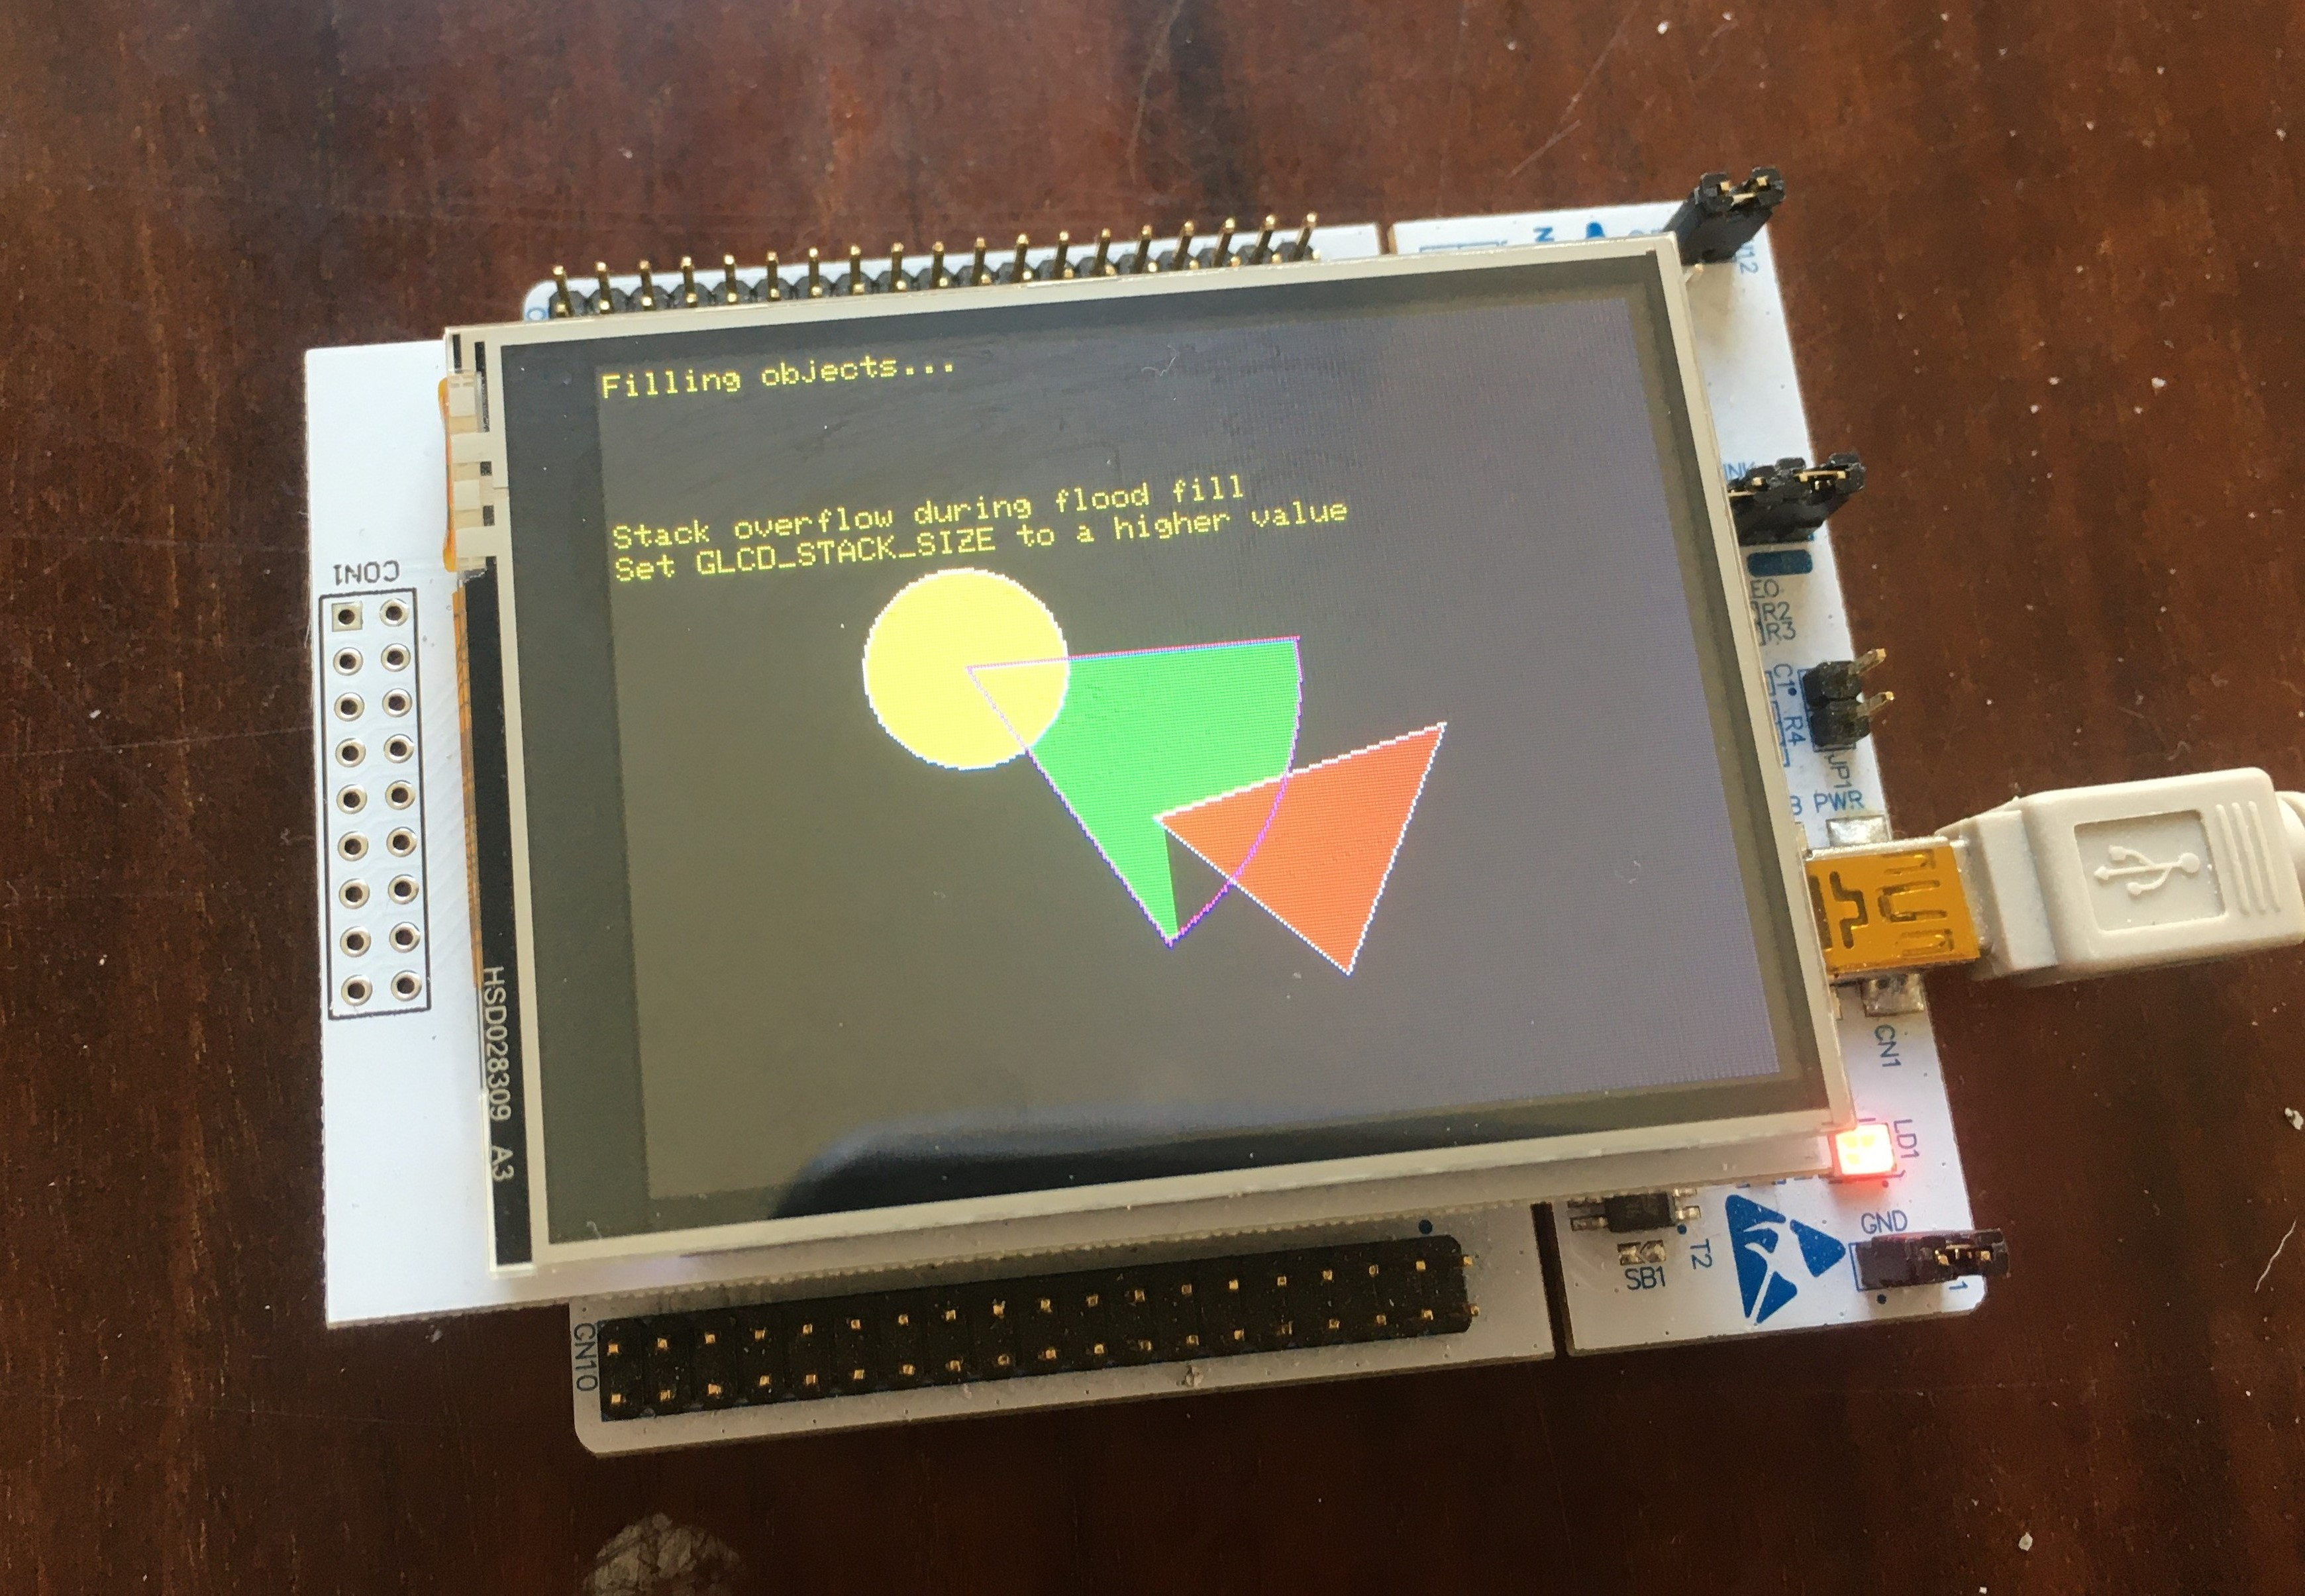
\includegraphics[width=0.7\textwidth]{glcd_demo}
\caption{Showing the VMA412 mounted on a STM32F446 Nucleo board.}
\label{fig:1}
\end{figure}


\section{Creating a project}
If you have downloaded the code from GitHub, then you already have all files needed. Just start STMCubeIDE and open the project. If you need to create a fresh project, make sure that you have selected the correct device. 
After creating a project, make sure that the files are in the appropriate folders. These files are:

\begin{lstlisting}
glcd_vma412.h           -- place in Core/Inc, definitions, typedefs etc
glcd_vma412.c           -- place in Core/Src, functions to call
touchscreen_vma412.h    -- place in Core/Inc, definitions, typedefs etc
touchscreen_vma412.c    -- place in Core/Src, functions to call
main.c                  -- place in Core/Src, demo using functions
dog_map.c               -- place in Core/Src, used in the demo
Fonts\FreeMono12pt7b.c  -- place in Core/Src/Fonts, used in demo
Fonts\FreeSerif12pt7b.c -- place in Core/Src/Fonts, used in demo
\end{lstlisting}

The files \lstinline|FreeMono12pt7b.c| and \lstinline|FreeSerif12pt7b.c| may be placed in the \lstinline|Core\Src| folder if needed.


\section{Running the demo}
If you have set up your project just start compilation using \texttt{Project}$\rightarrow$\texttt{Build Project}. Then start the the demo using \texttt{Run}$\rightarrow$\texttt{Run}. The demo starts by asking you to touch one of four rectangles to start the GLCD demo, the touchscreen demo, the rotation demo or the character set demo, see Figure~\ref{fig:2}. At the end of the GLCD demo, there will be a list of running times for selected graphic functions as can be seen in Figure~\ref{fig:3}.

\begin{figure}[!ht]
\centering
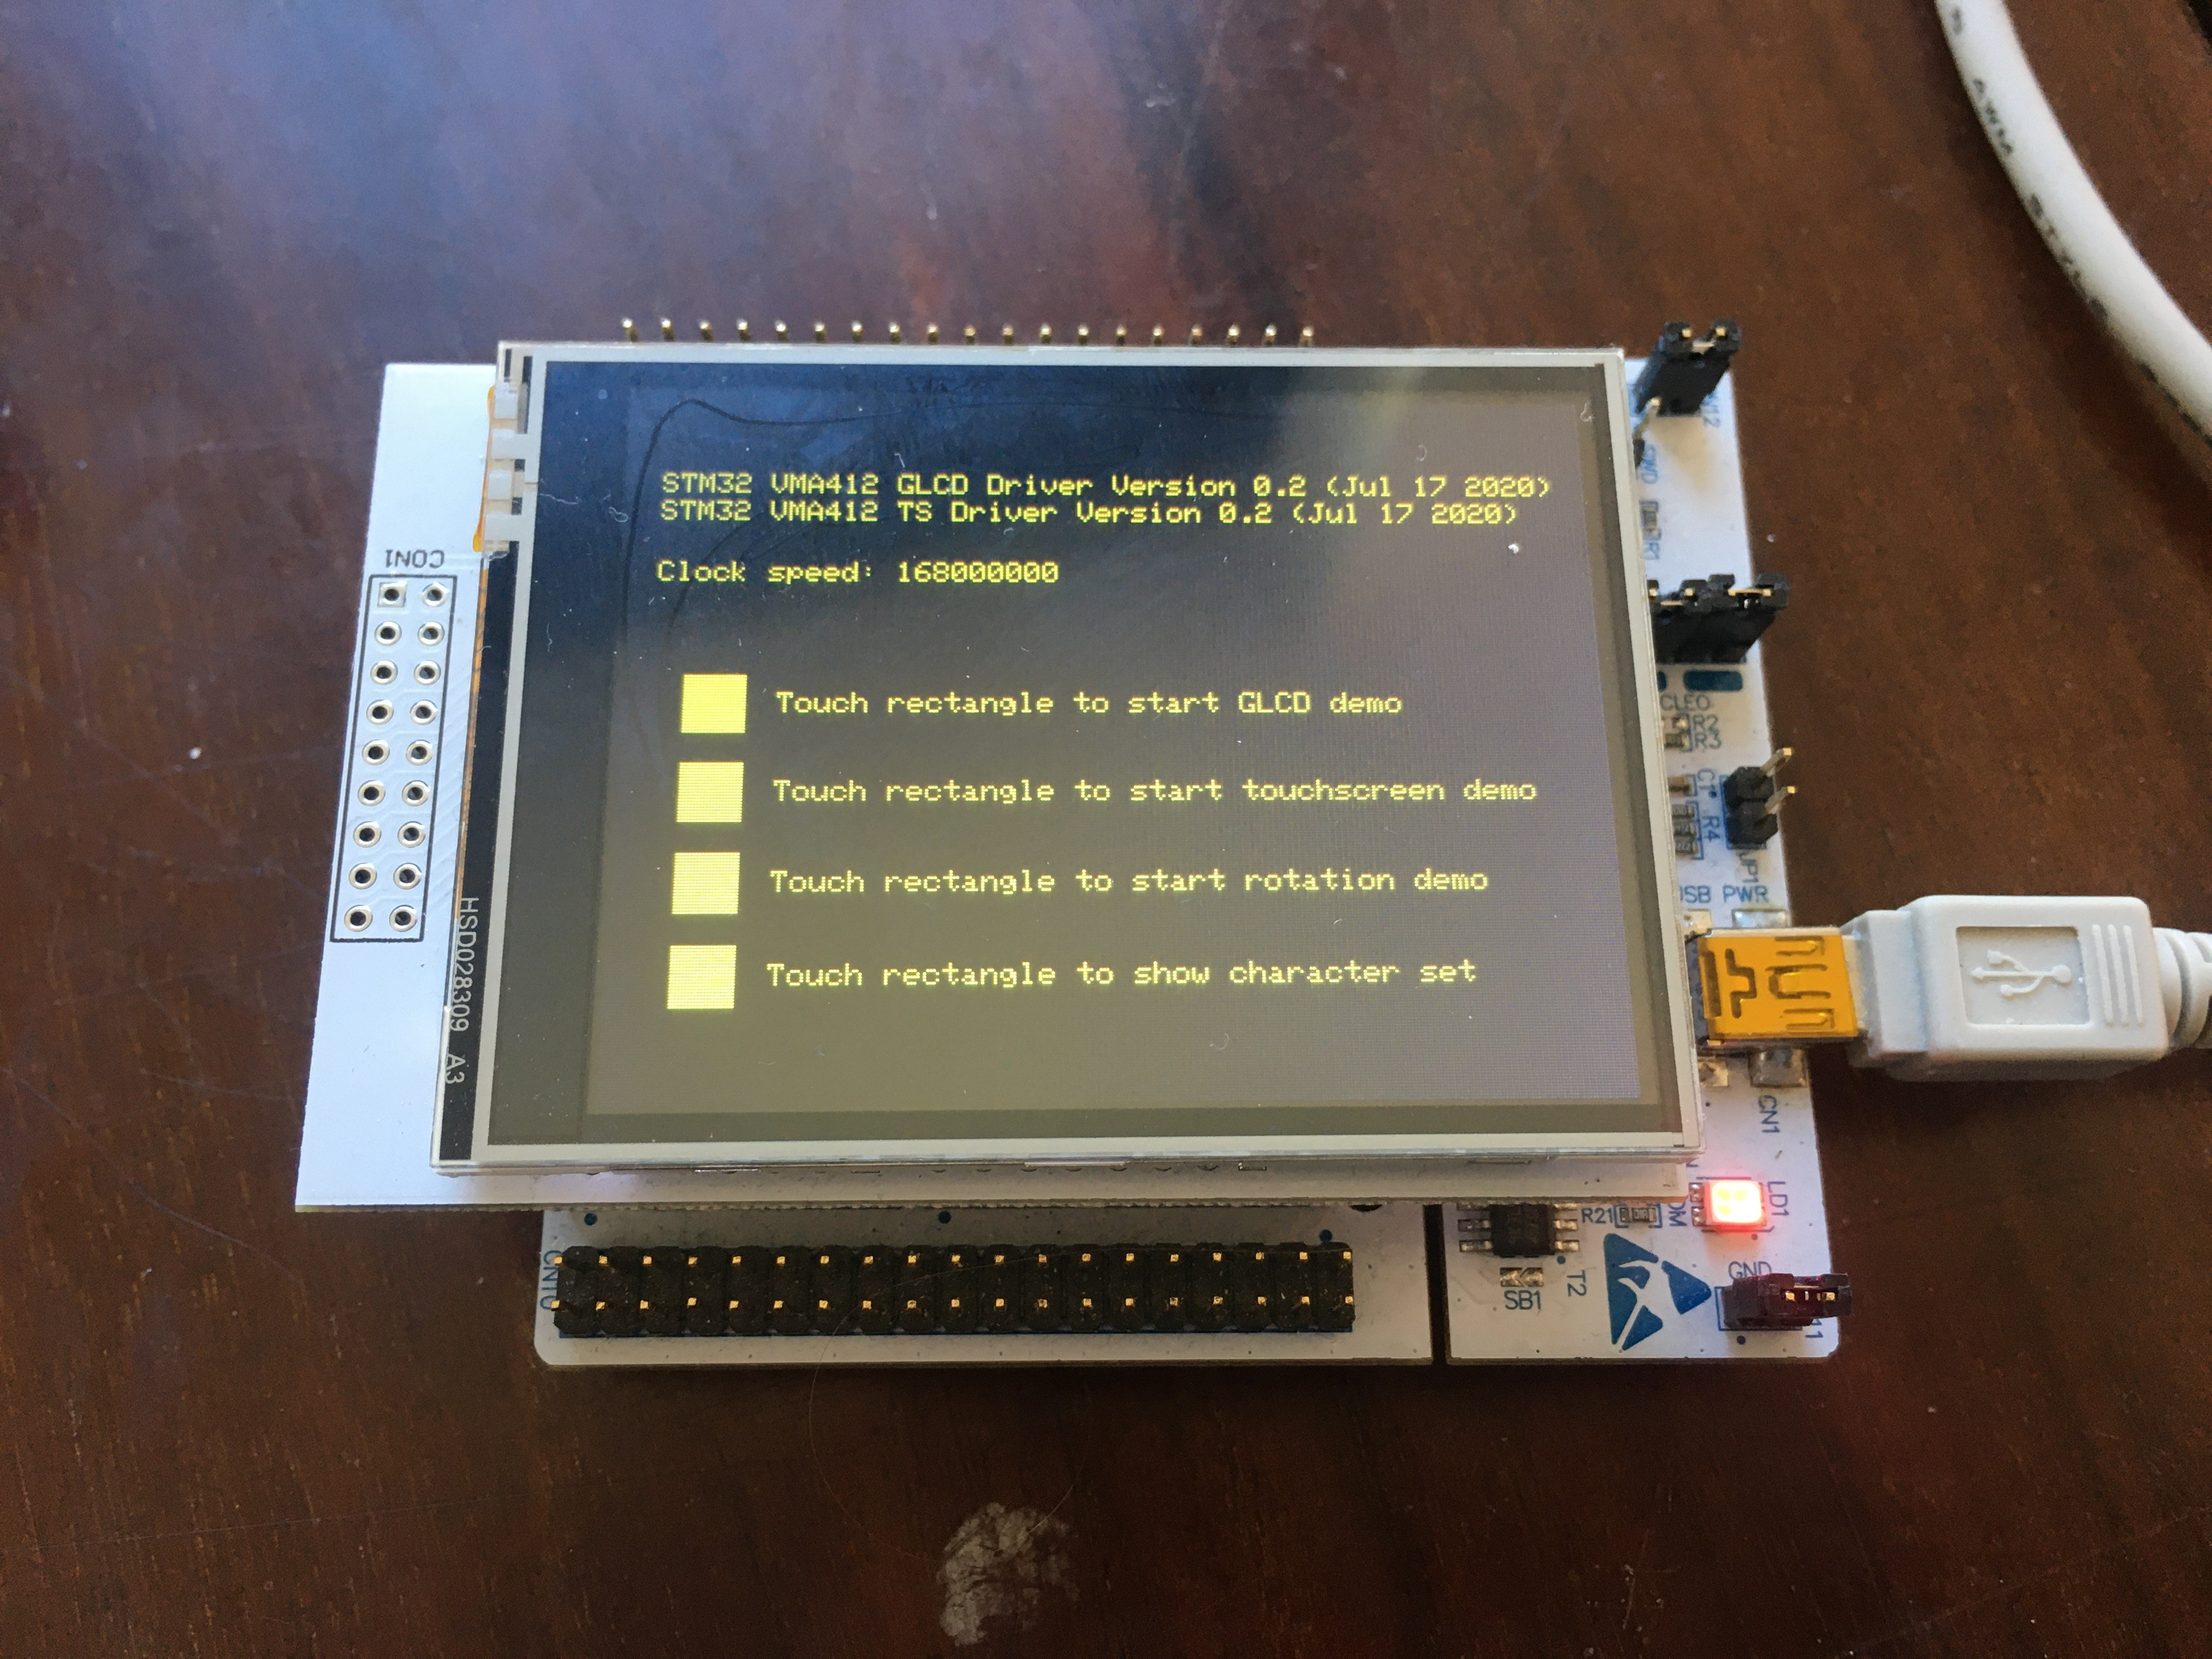
\includegraphics[width=0.7\textwidth]{start_demo}
\caption{Starting the demo.}
\label{fig:2}
\end{figure}

\begin{figure}[!ht]
\centering
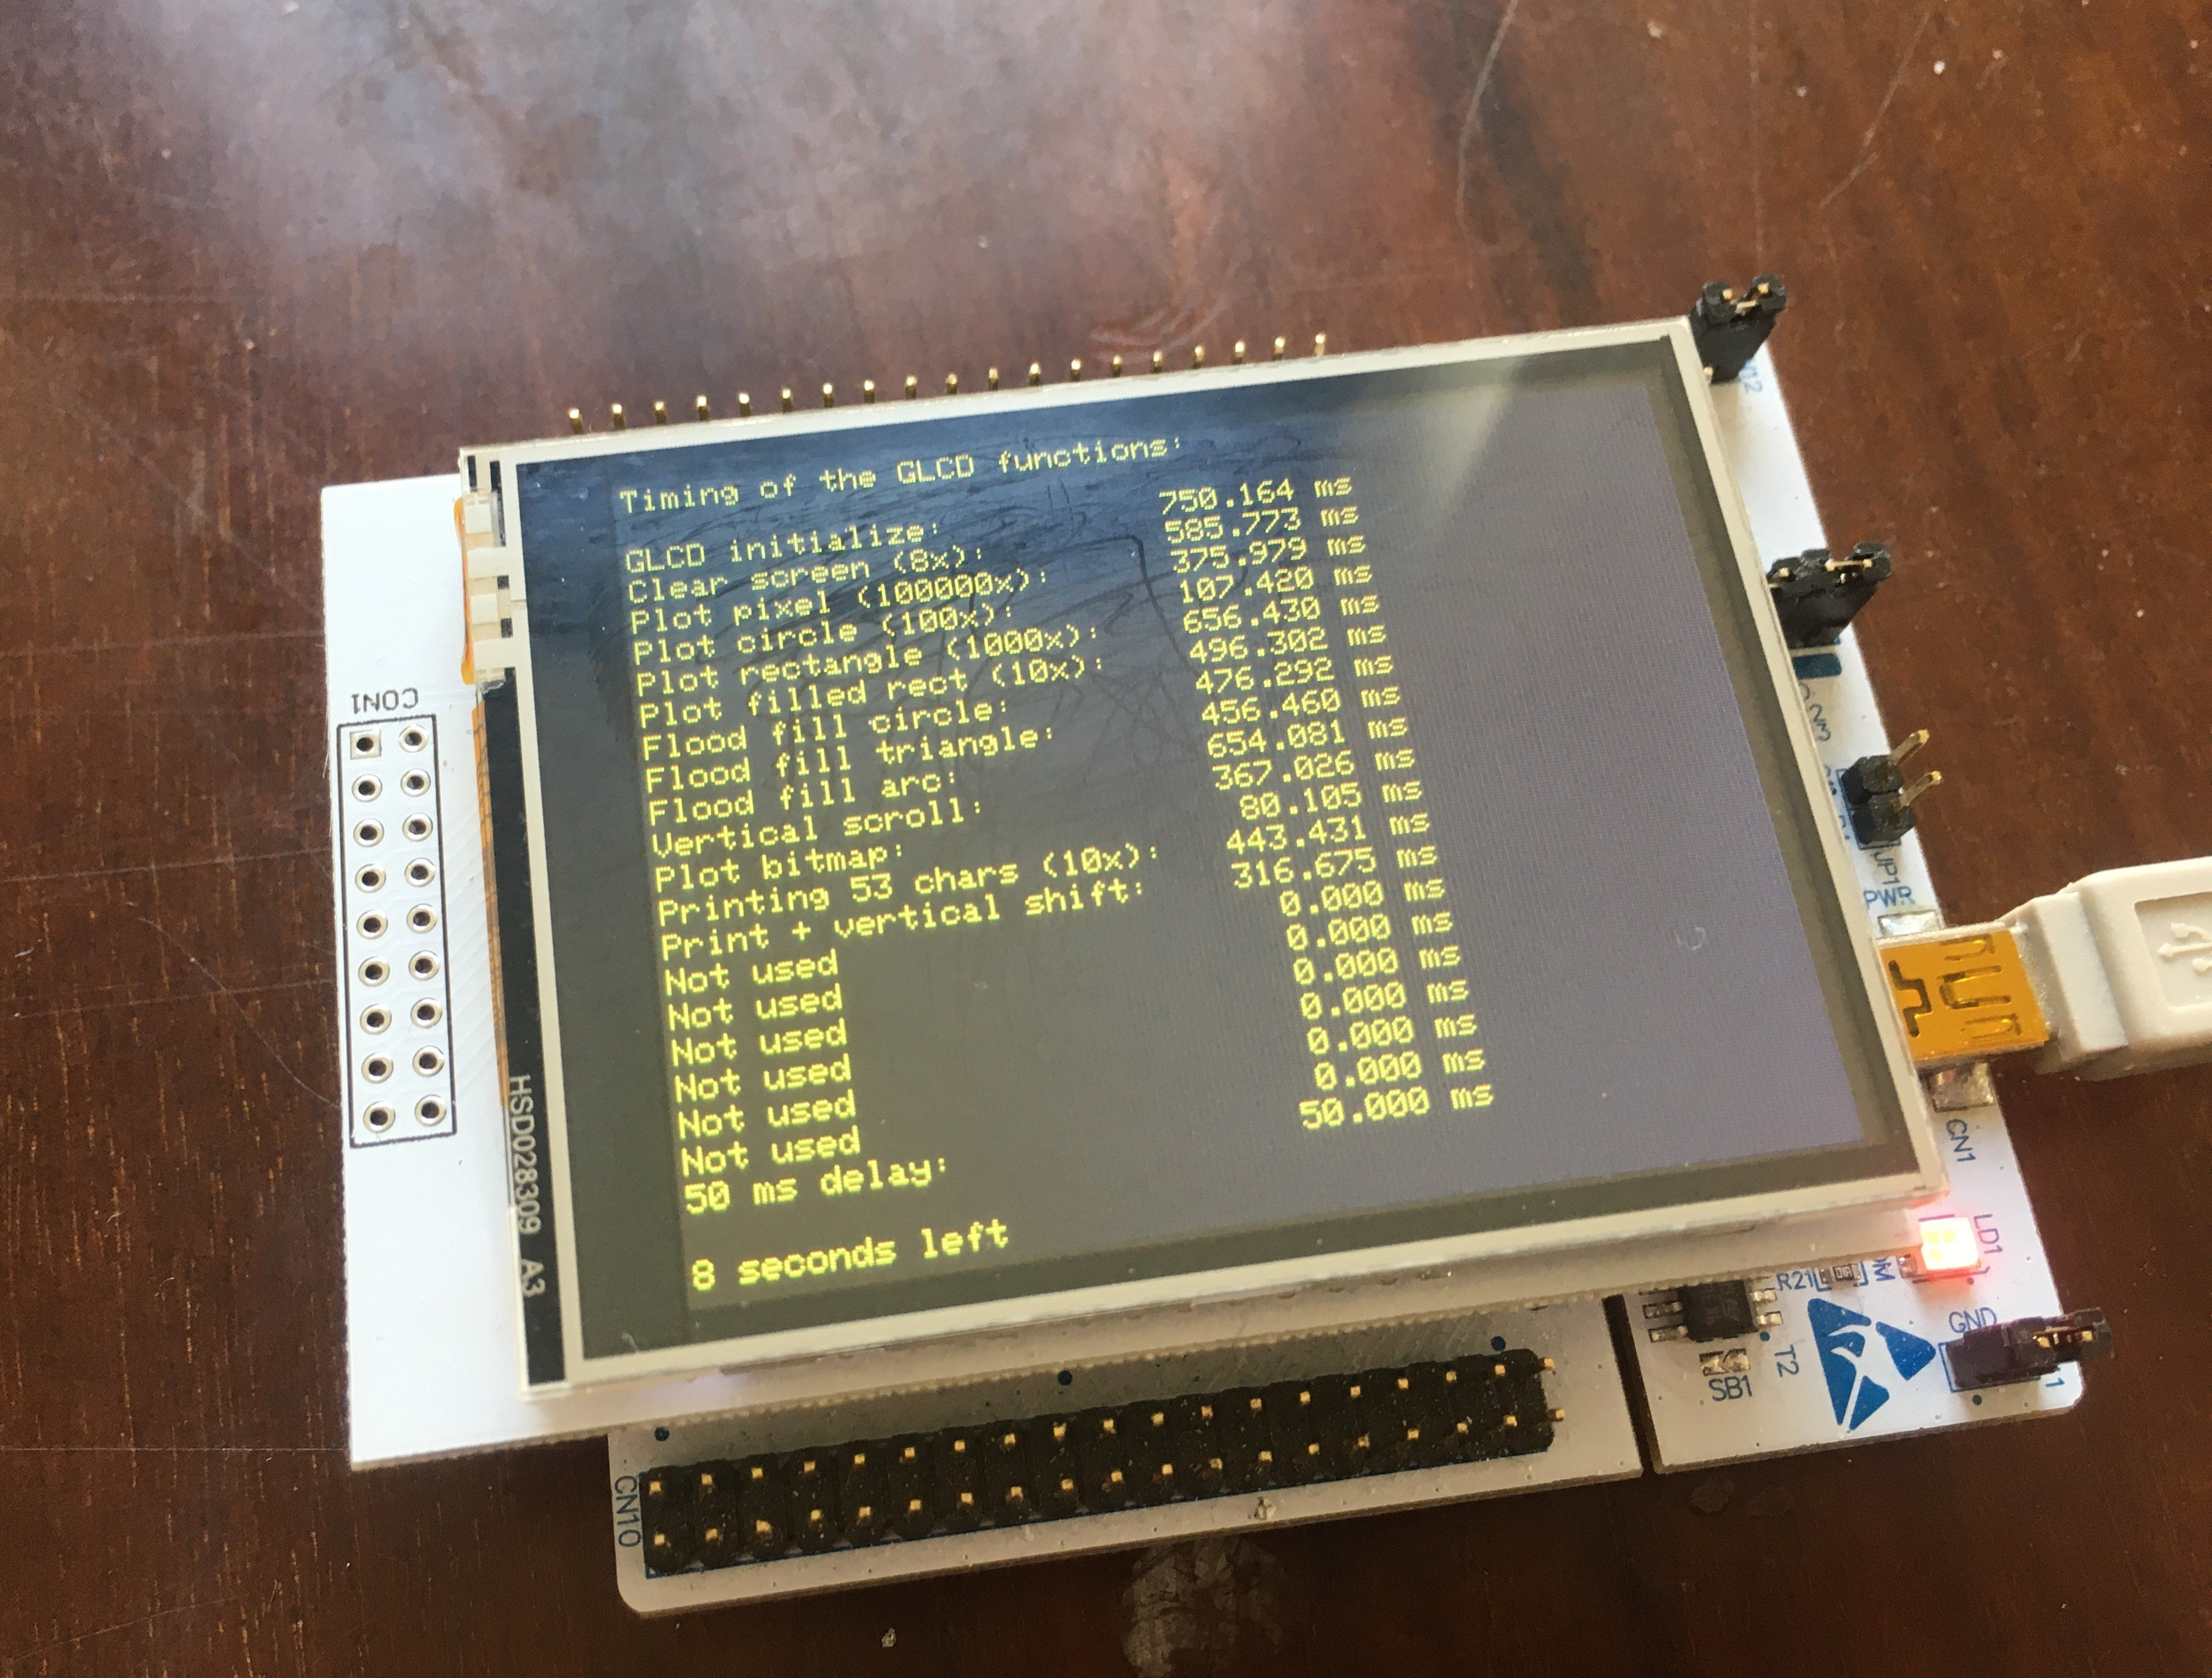
\includegraphics[width=0.7\textwidth]{times}
\caption{Displaying times for selected GLCD functions.}
\label{fig:3}
\end{figure}




\section{Graphic LCD}
This section discusses all functions for the Graphic LCD.

\subsection{X and Y coordinates, display orientation}
\index{Coordinate system}\index{Display orientation}
The X and Y coordinates use type \lstinline|int16_t| for their values, because some plotting functions involve negative values. Of course, real display coordinates only have positive values, or 0, and negative values for X or Y prohibit (partially) plotting. The display is set up in landscape where \lstinline|X| is between 0 and 319 and \lstinline|y| is between 0 and 239. Point (0,0) is in the upper left corner,
point (239,319) is in the lower right corner. The landscape orientation is with the SD-card socket to the right.
The display orientation can be changed, see $\S$~\ref{sec:rotdispl}.

\subsection{Other parameters}
Below is a summation of the types used:

\begin{itemize}
\item Radii, widths and heights use \lstinline|int16_t| as their type.
\item Characters are of type \lstinline|char| or \lstinline|uint8_t|.
\item Strings are of type \lstinline|char *| (or \lstinline|char []|).
\item Bitmaps and palettes are of type \lstinline|uint8_t|.
\item Colors are of type \lstinline|glcd_color_t|.
\item String spacings are of type \lstinline|glcd_spacing_t|.
\item Low-level buffer manipulations are of type \lstinline|glcd_buffer_t|.
\item Display inversions are of type \lstinline|glcd_display_inversion_t|.
\item Display idles are of type \lstinline|glcd_display_idle_t|.
\item Display on or offs are of type \lstinline|glcd_display_onoff_t|.
\item Display rotations are of type \lstinline|glcd_rotation_t|.
\end{itemize}

There are some other types, but they are normally not used.

\subsection{Color system}
\index{Color system}
The GLCD is set up to use the 18-bit color specification. This means that colors are specified with unsigned 32 bits. The specification is as follows:

Bits 31-24: ignored, should be kept at 0.\\
Bits 23-16: red -- only upper 6 bits are used\\
Bits 15-8: green -- only upper 6 bits are used\\
Bits 7-0: blue -- only upper 6 bits are used

Note: The 16-bit 5/6/5 color specification is \textbf{NOT} supported, but they can be converted. See $\S$~\ref{sec:convertcolors}.

Please note that although 8 bits per color can be specified, only the upper 6 bits of each color are used, since the display uses 18 bits of color infomation. The lower 2 bits of each color are ignored. This means that color \lstinline|0x000000| and \lstinline|0x000001| are displayed the same, but are different in compares.

The color is specified using the the type \lstinline|glcd_color_t|. Note: don't ever change the type \lstinline|glcd_color_t|.

\subsubsection{Predefined colors}
\index{Predefined colors}
There are some predefines colors:

\begin{lstlisting}
#define GLCD_COLOR_BLACK   (0x000000)
#define GLCD_COLOR_BLUE    (0x0000ff)
#define GLCD_COLOR_GREEN   (0x00ff00)
#define GLCD_COLOR_CYAN    (0x00ffff)
#define GLCD_COLOR_RED     (0xff0000)
#define GLCD_COLOR_MAGENTA (0xff00ff)
#define GLCD_COLOR_YELLOW  (0xffff00)
#define GLCD_COLOR_WHITE   (0xffffff)

#define GLCD_COLOR_NAVY        (0x000080)
#define GLCD_COLOR_DARKGREEN   (0x008000)
#define GLCD_COLOR_DARKCYAN    (0x008080)
#define GLCD_COLOR_MAROON      (0x800000)
#define GLCD_COLOR_PURPLE      (0x800080)
#define GLCD_COLOR_OLIVE       (0x808000)
#define GLCD_COLOR_LIGHTGREY   (0xC0C0C0)
#define GLCD_COLOR_ORANGE      (0xFFA500)
#define GLCD_COLOR_GREENYELLOW (0xADFF2F)
#define GLCD_COLOR_PINK        (0xFFC0CB)

#define GLCD_COLOR_GREY50  (0x808080)

/* THUAS default color */
#define GLCD_COLOR_THUASGREEN ((158<<16)|(167<<8)|0)
\end{lstlisting}

\subsubsection{Using your own color}
To use your own color, please use the color type \lstinline|glcd_color_t|:

\begin{lstlisting}
glcd_color_t SkyBlue2 = (126<<16)|(192<<8)|238
\end{lstlisting}

as taken for the \LaTeX\ \lstinline|xcolor| package (\url{https://www.ctan.org/pkg/xcolor}).

Note: don't ever change the type \lstinline|glcd_color_t|.

\subsection{GLCD Initialization}
First you have to set up the clock system used by the STM32F microcontroller. If you use the external clock generator, make sure that the value of \lstinline|HSE_VALUE| is set to the correct frequency. In the case of the Nucleo board it is 8000000 (8 MHz). This value is defined in \lstinline|stm32f4xx_hal_conf.h| and \lstinline|system_stm32f4xx.c|.

If you use the internal HSI (\lstinline|HSIVALUE|), the frequency is 16 MHz by default. Best is to set up the clock speed to the maximum frequency allowed by the microcontroller.

After the clock system is set up, initialize the display by calling the \lstinline|glcd_init()| function. After calling that function the display is initialized and ready for use.

\subsection{Very low level GLCD functions}

\subsubsection{Setting the write delay}
\label{sec:writedelay}
\ifunc{glcd\_set\_write\_pulse\_delay}
\textbf{Note:} use with care.\\
Sets the delay for write actions. There is no need to call this function as the correct timing is calculated according to the system clock speed after the clock system is set up, but you can tweak this value to get maximum performance. \lstinline|delay| must be greater than 0. The function prototype is:
\begin{lstlisting}
void glcd_set_write_pulse_delay(uint32_t delay);
\end{lstlisting}

\subsubsection{Setting the read delay}
\label{sec:readdelay}
\ifunc{glcd\_set\_read\_pulse\_delay}
\textbf{Note:} use with care.\\
Sets the delay for read actions. There is no need to call this function as the correct timing is calculated according to the system clock speed after the clock system is set up, but you can tweak this value to get maximum performance. \lstinline|delay| must be greater than 0. The function prototype is:

\begin{lstlisting}
void glcd_set_read_pulse_delay(uint32_t delay);
\end{lstlisting}

\subsection{GLCD low level functions}
\ifunc{glcd\_read\_terminate}
There are a number of low level functions. They are normally not needed.

\subsubsection{Reading data from the display}

To read data from the display, use the function \lstinline|glcd_read_terminate|. Reading is explicitly terminated. The function prototype is:

\begin{lstlisting}
void glcd_read_terminate(uint16_t cmd,            // The command
                         uint16_t amount,         // Amount of data
                         glcd_buffer_t data[]);   // The buffer
\end{lstlisting}

Note: if you read pixel color information (one or more pixels), the first element of the buffer is useless information.

\subsubsection{Writing data to the display}
\ifunc{glcd\_write}
Writes data to the display, no explicit terminate. This means that multiple writes can be done in sequence.
\begin{lstlisting}
void glcd_write(uint16_t cmd,                     // The command
                uint16_t amount,                  // Amount of data
                const glcd_buffer_t data[]);      // The buffer
\end{lstlisting}

\subsubsection{Explicit terminating a write}
\ifunc{glcd\_terminate\_write}
Terminates a write:
\begin{lstlisting}
void glcd_terminate_write(void);
\end{lstlisting}

\subsubsection{Changing the buffer type}
\index{Changing buffer type}
\label{sec:changebuf}
The low level functions use an internal buffer. The buffer is of type \lstinline|glcd_buffer_t|. This normally set to an unsigned 16-bit size. This size can be changed, see $\S$~\ref{sec:taylorbuffer}.

 
\subsection{GLCD high level commands}

\subsubsection{Initialize display}
Note: call this function \textbf{after} the clock system is set up.

This function must be called after the clock system is set up and before using any other GLCD functions. The function prototype is:
\begin{lstlisting}
void glcd_init(void);
\end{lstlisting}

\subsubsection{Delay}
\ifunc{glcd\_delay\_ms}
To delay your applications (in milliseconds), use :

\begin{lstlisting}
void glcd_delay_ms(uint32_t delay);
\end{lstlisting}

\subsubsection{Rotating the display}
\ifunc{glcd\_setrotation}
\label{sec:rotdispl}

To set the rotation of the display, use:
\begin{lstlisting}
void glcd_setrotation(glcd_rotation_t rot);
\end{lstlisting}

Where \lstinline|rot| is one of:

\begin{lstlisting}
GLCD_DISPLAY_ROT0           // Standard landscape, default
GLCD_DISPLAY_ROT90          // Rotate 90 degrees counter clockwise
GLCD_DISPLAY_ROT180         // Rotate 180 degrees counter clockwise
GLCD_DISPLAY_ROT270         // Rotate 270 degrees counter clockwise
\end{lstlisting}

Notes on rotation:

When you rotate the display, the current display contents are neighter deleted nor rotated. You have to clear the display explicitly.

The default rotation is 0$^\circ$. The display is in landscape with the SD-card socket on the right of the display. A rotation of 90$^\circ$ sets the display is portrait mode with the SD-card socket at the bottom of the display. A rotation of 180$^\circ$ sets the display in landscape mode with the SD-card socket to the left of the Display. A rotation of 270$^\circ$ set the display in portrait mode with the SD-card socket at the top of the display.

To be compatible with Arduino-based software, set the rotation to 90$^\circ$.

Note: the touchscreen is \textbf{not} rotated. The touchscreen functions are setup for the standard rotation of 0$^\circ$. How to handle the touchscreen in case of rotated displays, see $\S$~\ref{sec:rottouch}.

\subsubsection{Clear the display}
\ifunc{glcd\_cls}

To clear the display with a color, use:
\begin{lstlisting}
void glcd_cls(glcd_color_t color);
\end{lstlisting}

\subsubsection{Plot a pixel}
\ifunc{glcd\_plotpixel}
To plot a pixel, use:
\begin{lstlisting}
void glcd_plotpixel(int16_t x,            // x coordinate
                    int16_t y,            // y coordinate
                    glcd_color_t color);  // color
\end{lstlisting}

Note: if \lstinline|x| is greater than the width of the display minus 1, the pixel is not plotted.\\
Note: if \lstinline|x| is less than 0, the pixel is not plotted.\\
Note: if \lstinline|y| is greater than the height of the display, minus 1, the pixel is not plotted.\\
Note: if \lstinline|y| is less than 0, minus 1, the pixel is not plotted.\\

\subsubsection{Read a pixel}
\ifunc{glcd\_readpixel}
To read a pixel (getting color information) in \lstinline|glcd_color_t| use:

\begin{lstlisting}
glcd_color_t glcd_readpixel(int16_t x,   // x coordinate
                            int16_t y);  // y coordinate
\end{lstlisting}

Note: if \lstinline|x| is greater that the width of the display minus 1, the returned color is undefined.\\
Note: if \lstinline|y| is greater that the height of the display, minus 1, the returned color is undefined.\\
Note: if \lstinline|x| or \lstinline|y| is less than 0, \lstinline|GLCD_COLOR_BLACK| is returned.

\subsubsection{Plot a horizontal line}
\ifunc{glcd\_plothorizontalline}
To plot a horizontal line (fast), use:
\begin{lstlisting}
void glcd_plothorizontalline(int16_t x,            // x coordinate
                             int16_t y,            // y coordinate
                             int16_t w,            // width
                             glcd_color_t color);  // color
\end{lstlisting}

Note: if \lstinline|x+w| is greater than the width of the display minus 1, the pixels in excess are not plotted.

\subsubsection{Plot a vertical line}
\ifunc{glcd\_plotverticalline}
To plot a vertical line (fast), use:
\begin{lstlisting}
void glcd_plotverticalline(int16_t x               // x coordinate
                           int16_t y,              // y coordinate
                           int16_t h,              // height
                           glcd_color_t color);    // color
\end{lstlisting}
Note: if \lstinline|y+h| is greater than the height of the display minus 1, the pixels in excess are not plotted.

\subsubsection{Plot a line with any angle and length}
\ifunc{glcd\_plotline}
To plot a line with any angle and length, use:
\begin{lstlisting}
void glcd_plotline(int16_t x0,            // x start point
                   int16_t y0,            // y start point
                   int16_t x1,            // x end point
                   int16_t y1,            // y end point
                   glcd_color_t color);   // color
\end{lstlisting}

Note: the part of the line that is exceeding the dimensions of the display are not plotted.

\subsubsection{Plot a rectangle}
\ifunc{glcd\_plotrect}
To plot a rectangle, use:
\begin{lstlisting}
void glcd_plotrect(int16_t x,              // x coordinate
                   int16_t y,              // y coordinate
                   int16_t w,              // width
                   int16_t h,              // height
                   glcd_color_t color);    // color
\end{lstlisting}

Note: \lstinline|x| and \lstinline|y| specify the upper left corner.

\subsubsection{Plot a filled rectangle}
\ifunc{glcd\_plotrectfill}
To plot a filled rectangle, use:
\begin{lstlisting}
void glcd_plotrectfill(int16_t x,             // x coordinate
                       int16_t y,             // y coordinate
                       int16_t w,             // width
                       int16_t h,             // height
                       glcd_color_t color);   // color
\end{lstlisting}

Note: \lstinline|x| and \lstinline|y| specify the upper left corner.

\subsubsection{Plot a rectangle with rounded corners}
\ifunc{glcd\_plotrectrounded}
To plot a rectangle with rounded corners, use:

\begin{lstlisting}
void glcd_plotrectrounded(int16_t x,            // x coordinate
                          int16_t y,            // y coordinate
                          int16_t w,            // width
                          int16_t h,            // height
                          int16_t r,            // radius
                          glcd_color_t color);  // color
\end{lstlisting}

Note: \lstinline|x| and \lstinline|y| specify the upper left corner as plotted with \lstinline|glcd_plotrect|. \\
Note: \lstinline|r| must be greater than 0.

\subsubsection{Plot a filled rectangle with rounded corners}
\ifunc{glcd\_plotrectroundedfill}
To plot a filled rectangle with rounded corners, use:

\begin{lstlisting}
void glcd_plotrectroundedfill(int16_t x,            // x coordinate
                              int16_t y,            // y coordinate
                              int16_t w,            // width
                              int16_t h,            // height
                              int16_t r,            // radius
                              glcd_color_t color);  // color
\end{lstlisting}

Note: \lstinline|x| and \lstinline|y| specify the upper left corner as plotted with \lstinline|glcd_plotrect|.\\
Note: \lstinline|r| must be greater than 0.

\subsubsection{Plot a circle}
\ifunc{glcd\_plotcircle}
To plot a circle, use:
\begin{lstlisting}
void glcd_plotcircle(int16_t x0,              // center x coordinate
                     int16_t y0,              // center y coordinate
                     int16_t r,               // radius
                     glcd_color_t color);     // color
\end{lstlisting}

Note: \lstinline|r| must be greater than 0.


\subsubsection{Plot a filled circle}
\ifunc{glcd\_plotcirclefill}
To plot a filled circle, use:
\begin{lstlisting}
void glcd_plotcirclefill(int16_t x0,              // center x coordinate
                         int16_t y0,              // center y coordinate
                         int16_t r,               // radius
                         glcd_color_t color);     // color
\end{lstlisting}

Note: \lstinline|r| must be greater than 0.

\subsubsection{Plot quarters of a circle}
\ifunc{glcd\_plotcirclequarter}
To plot quarters of a circle, use:
\begin{lstlisting}
void glcd_plotcirclequarter(int16_t x0,                // center x
                            int16_t y0,                // center y
                            int16_t r,                 // radius
                            glcd_corner_t cornername,  // corners
                            glcd_color_t color);       // color
\end{lstlisting}

Note: this function doesn't plot the start and end points.\\
Note: \lstinline|r| must be greater than 0.\\
Note: \lstinline|cornername| is one of or a composition of: 
\lstinline|GLCD_CORNER_UPPER_LEFT|,\\ \lstinline|GLCD_CORNER_UPPER_RIGHT|, \lstinline|GLCD_CORNER_LOWER_RIGHT| and \lstinline|GLCD_CORNER_LOWER_LEFT|

\subsubsection{Plot and fill left and/or right halves of a circle}
\ifunc{glcd\_plotcirclehalffill}
To plot and fill left and/or right halves of a circle, use:

\begin{lstlisting}
void glcd_plotcirclehalffill(int16_t x0,                  // center x
                             int16_t y0,                  // center y
                             int16_t r,                   // radius
                             glcd_cornerhalves_t corners, // see notes
                             int16_t delta,               // see notes
                             glcd_color_t color);         // color
\end{lstlisting}

Notes \lstinline|delta| is the squeeze factor, positive squeezes left/right, negative squeezes top/bottom, 0 for plain circle.\\
Note: \lstinline|r| must be greater than 0.\\
Note: \lstinline|corners| is one of \lstinline|GLCD_CORNER_LEFT_HALF|, \lstinline|GLCD_CORNER_RIGHT_HALF| and\\ \lstinline|GLCD_CORNER_BOTH|.\\
Note: doesn't plot the outer top-to-bottom vertical line. 

\subsubsection{Plot a triangle}
\ifunc{glcd\_plottriangle}
To plot a triangle, use:

\begin{lstlisting}
void glcd_plottriangle(int16_t x0,           // start x
                       int16_t y0,           // start y
                       int16_t x1,           // second x
                       int16_t y1,           // second y
                       int16_t x2,           // third x
                       int16_t y2,           // third y
                       glcd_color_t color);  // color
\end{lstlisting}

\subsubsection{Plot a filled triangle}
\ifunc{glcd\_plottrianglefill}
To plot a filled triangle, use:

\begin{lstlisting}
void glcd_plottrianglefill(int16_t x0,            // first x
                           int16_t y0,            // first y
                           int16_t x1,            // second x
                           int16_t y1,            // second y
                           int16_t x2,            // third x
                           int16_t y2,            // third y
                           glcd_color_t color);   // color

\end{lstlisting}

\subsubsection{Plot a regular polygon}
\label{sec:regpoly}
\ifunc{glcd\_plotregularpolygon}
To plot a regular polygon, with evenly spaced sides, use

\begin{lstlisting}
void glcd_plotregularpolygon(int16_t xc,            // center x
                             int16_t yc,            // center y
                             int16_t r,             // radius
                             int16_t sides,         // number of sides
                             float displ,           // angle displacement
                             glcd_color_t color);   // color
\end{lstlisting}

Note: this function is only available is \lstinline|GLCD_USE_REGULAR_POLYGON| is defined.\\
Note: \lstinline|r| must be greater than 0.\\
Note: this function uses \lstinline|sinf| and \lstinline|cosf| math functions, using the onboard FPU.\\
Note: \lstinline|displ| is angle displacement from the positive x axis downwards.\\
Note: if \lstinline|sides| is less than 1, nothing is plotted.\\
Note: if \lstinline|sides| is 1, a point is plotted on (xc + r$\cdot$cos(angle), yx+r$\cdot$cos(angle)).\\
Note: if \lstinline|sides| is 2, a line is plotted between (xc + r$\cdot$cos(angle), yx+r$\cdot$cos(angle)) and (xc + r$\cdot$cos($\pi$+angle), yx+r$\cdot$cos($\pi$+angle)).

\subsubsection{Plot a filled regular polygon}
\ifunc{glcd\_plotregularpolygonfill}
To plot a filled regular polygon, with evenly spaced sides, use

\begin{lstlisting}
void glcd_plotregularpolygonfill(int16_t xc,           // center x
                                 int16_t yc,           // center y
                                 int16_t r,            // radius
                                 int16_t sides,        // number of sides
                                 float displ,           // angle displacement
                                 glcd_color_t color);   // color
\end{lstlisting}

Note: see $\S$~\ref{sec:regpoly}.\\
Note: this function uses the filled triangle function to do its job.

\subsubsection{Plot an arc}\textbf{}
\ifunc{glcd\_plotarc}
To plot an arc, use:
\begin{lstlisting}
void glcd_plotarc(int16_t xc,                 // center x coordinate
                  int16_t yc,                 // center y coordinate
                  int16_t r,                  // radius
                  float start,                // start angle in degrees
                  float stop,                 // stop angle in degrees
                  glcd_color_t color);        // color
\end{lstlisting}

Note: this function is only available if \lstinline|GLCD_USE_ARC| is defined.\\
Note: \lstinline|r| must be greater than 0. \\
Note: this function uses \lstinline|sinf| and \lstinline|cosf| math functions, using the onboard FPU.\\
Note: start and stop angles are counted from the positive x axis downwards.

\subsubsection{Plot a 2-color bitmap}
\ifunc{glcd\_plotbitmap}
To plot a 2-color bitmap with explicit defined colors, use:
\begin{lstlisting}
void glcd_plotbitmap(int16_t x,               // x coordinate
                     int16_t y,               // y coordinate
                     const uint8_t bitmap[],  // the bitmap, see note
                     int16_t w,               // width
                     int16_t h,               // height
                     glcd_color_t color,      // color
                     glcd_color_t bg);        // background color
\end{lstlisting}

Note: \lstinline|bitmap| consists of bytes (\lstinline|uint8_t|). A 1 in a byte is converted to \lstinline|color|, a 0 in a byte is converted to \lstinline|bg|.\\
Note: a full 320x240 pixels image needs 9728 bytes of ROM.\\
Note: you will get compiler warnings if your bitmap is in RAM, because \lstinline|bitmap| is qualified as \lstinline|const|.

Note: if you need to convert your image to a 2-bit color bitmap, have a look at \url{https://lvgl.io/tools/imageconverter}.

\subsubsection{Plot a 256-color indexed bitmap}
\ifunc{glcd\_plotbitmap8bpp}
To plot a 256-color indexed bitmap, use:
\begin{lstlisting}
void glcd_plotbitmap8bpp(int16_t x,                // x start point
                         int16_t y,                // y start point
                         int16_t w,                // width
                         int16_t h,                // height
                         const uint8_t *pic,       // start of image
                         const uint8_t *palette);  // start of palette
\end{lstlisting}

Note: each pixel is specified with a byte (\lstinline|uint8_t|). This is an index into the palette.\\
Note: each color is specified with a 32-bit RGB color specification. This means that each color takes up four bytes and the total palette size is 1024 bytes. The byte order for each indexed color is as follows: first byte is red, second byte is green, third byte is blue, fourth byte is not used.\\
Note: is \lstinline|palette| is equal to \lstinline|NULL| then the palette is at the start of the image and the image bytes follow the palette.\\
Note: you will get compiler warnings if your bitmap is in RAM, because \lstinline|bitmap| is qualified as \lstinline|const|.\\
Note: you will get compiler warnings if your palette is in RAM, because \lstinline|palette| is qualified as \lstinline|const|.\\
Note: a full 320x240 pixels image needs 77824 bytes of ROM.\\
Note: if you need to convert your image to a 256-color indexed image, have a look at \url{https://lvgl.io/tools/imageconverter}.

\subsubsection{Display inversion}
\ifunc{glcd\_inversion}
Sets the display inversion (or not):
\begin{lstlisting}
void glcd_inversion(glcd_display_inversion_t what);
\end{lstlisting}

Note: \lstinline|what| is one of:
\begin{lstlisting}
GLCD_DISPLAY_INVERSION_OFF
GLCD_DISPLAY_INVERSION_ON
\end{lstlisting}

\subsubsection{Display idle}
\ifunc{glcd\_idle}
Set the display to idle (or not):
\begin{lstlisting}
void glcd_idle(glcd_display_idle_t what);
\end{lstlisting}

Note: \lstinline|what| is one of:

\begin{lstlisting}
GLCD_DISPLAY_IDLE_OFF
GLCD_DISPLAY_IDLE_ON
\end{lstlisting}

\subsubsection{Display on or off}
\ifunc{glcd\_display}
Sets the display on or off:
\begin{lstlisting}
void glcd_display(glcd_display_t what);
\end{lstlisting}

Note: \lstinline|what| is one of

\begin{lstlisting}
GLCD_DISPLAY_OFF
GLCD_DISPLAY_ON
\end{lstlisting}

\subsubsection{Flood fill an object}
\ifunc{glcd\_floodfill}
Flood fill an object using a software stack based approach:
\begin{lstlisting}
void glcd_floodfill(int16_t xs,                  // x start point
                    int16_t ys,                  // y start point
                    glcd_color_t fillColor,      // color for pixel == 1
                    glcd_color_t defaultColor);  // color for pixel == 0
\end{lstlisting}

Note: this function is only available if \lstinline|GLCD_USE_FLOOD_FILL| is defined.\\
Note: set \lstinline|GLCD_STACK_SIZE| to an appropiate value.\\
Note: if you have problems filling an object increase the value of \lstinline|GLCD_STACK_SIZE|.\\
Note: the stack uses unsigned 32-bit entries so the complete stack uses \lstinline|GLCD_STACK_SIZE|*4 bytes of RAM.\\
Note: filling object can be slow.\\
Note: make sure that the start coordinate is a valid display coordinate, otherwise nothing is filled.

\subsubsection{Scroll the display vertical upwards}
\ifunc{glcd\_scrollvertical}
To scroll the display vertical a number of lines, use:
\begin{lstlisting}
void glcd_scrollvertical(int16_t lines);   // lines to scroll upwards
\end{lstlisting}

Note: \lstinline|lines| must be greater than 0.\\
Note: this is a software based scroll, be is inherently slow.\\
Note: The lines are scrolled upwards off the display (no rotation), and the vacant lines are left untouched.

\subsubsection{Plot a character using buildin font}
\ifunc{glcd\_plotchar}
To plot a character using the buildin font (5x8), use:
\begin{lstlisting}
void glcd_plotchar(int16_t x,             // x coordinate
                   int16_t y,             // y coordinate
                   uint8_t c,             // character (0-255)
                   glcd_color_t color,    // color
                   glcd_color_t bg);      // background color
\end{lstlisting}

Note: character is one of 0 -- 255 (no special C treatment).\\
Note: if \lstinline|color| is equal to \lstinline|bg| then pixels having background color are not plotted.\\
Note: \lstinline|x| and \lstinline|y| specify the upper-left corner of the character, and the character is plotted towards positive x and y.

\subsubsection{Plot a string using buildin font}
\ifunc{glcd\_plotstring}
To plot a string using the buildin font, use:
\begin{lstlisting}
void glcd_plotstring(int16_t x,                  // x coordinate
                     int16_t y,                  // y coordinate
                     char str[],                 // the string
                     glcd_color_t color,         // color
                     glcd_color_t bg,            // background color
                     glcd_spacing_t spacing);    // spacing
\end{lstlisting}

Note: a \lstinline|\0| terminates a string (as in C). This means that buildin character 0 cannot be plotted.\\
Note: if \lstinline|color| is equal to \lstinline|bg| then pixels having background color are not plotted.\\
Note: \lstinline|x| and \lstinline|y| specify the upper-left corner of the first character, and characters are plotted towards positive x and and y.\\
Note: \lstinline|spacing| is one of:
\begin{lstlisting}
GLCD_STRING_CONDENSED  // zero pixels apart
GLCD_STRING_NORMAL     // magnification x pixel apart
GLCD_STRING_WIDE       // 2 times magnification x pixels apart
\end{lstlisting}

\subsubsection{Set magnification for character plotting}
\ifunc{glcd\_setcharsize}
To set the magnification for character plotting, use:

\begin{lstlisting}
void glcd_setcharsize(int16_t sizx,       -- x magnigication
                      int16_t sizy);      -- y magnification
\end{lstlisting}

Note: \lstinline|x| and/or \lstinline|y| must be greater that 0.\\
Note: sensible values are 1, 2, 3 and 4.\\
Note: not used for console based printing. Console based printing is always with magnification 1 for x and y.

\subsubsection{Set a character layout}
\ifunc{glcd\_setcharlayout}
To set a character layout for the builtin font, use:

\begin{lstlisting}
void glcd_setcharlayout(uint16_t c,       // the character
                        uint16_t byte0,   // first byte
                        uint16_t byte1,
                        uint16_t byte2,
                        uint16_t byte3,
                        uint16_t byte4);  // last byte
\end{lstlisting}

Note: only usable for the builtin font.\\
Note: the character table has to be in RAM. See $\S$~\ref{sec:glcdtaylor}.\\
Note: \lstinline|c| must be 0 -- 255.\\
Note: charaters of the builtin font take up 5x8 pixels. Each byte specifies one column of 8 pixels. The first byte specifies the left most column. Subsequent bytes specify columns to the left of the previous one. The LSB of the bytes specify the top most pixel of a column. The MSB of the bytes specify the bottom most pixel. A one bit specifies a pixel to be drawn in foreground color, a zero bit specifies a pixel to be drawn in background color. Although the parameters are typed \lstinline|uint16_t|, only the lower 8 bits are used.

\subsubsection{Console based character printing}
\ifunc{glcd\_putchar}
\label{sec:consolebasedcharacterprinting}
To use a simple console based character printing, use:
\begin{lstlisting}
void glcd_putchar(char c);
\end{lstlisting}

Note: characters are printed in yellow, background is black.\\
Note: \lstinline|\f| (form feed) clears the display.\\
Note: \lstinline|\n| returns and goes to the next line, may cause a vertical shift.\\
Note: \lstinline|\r| returns to the beginning of the line.\\
Note: \lstinline|\b| erases last character and goes one character back (ultimate to the beginning of the line).\\
Note: \lstinline|\t| creates tab stops at 8 character intervals\\Note: all other characters are printed using the internal font.\\
Note: if a character ``falls off'' the display, line wrap will be used, may cause a vertical shift.\\
Note: this function is aware of the current display rotation.

\subsubsection{Console based string printing}
\ifunc{glcd\_puts}
To use a simple console based string printing use:
\begin{lstlisting}
void glcd_puts(char str[]);
\end{lstlisting}

Note: \lstinline|str| is terminated with \lstinline|\0| (as in C).\\
Note: see $\S$\ref{sec:consolebasedcharacterprinting} for character handling.\\
Note: if \lstinline|str| equals \lstinline|NULL|, then \lstinline|(null)| is printed.

\subsubsection{Activate an alternative font}
\ifunc{glcd\_setfont}
To activate an alternative font, use

\begin{lstlisting}
void glcd_setfont(const GFXfont *f);  -- f is pointer to font handle
\end{lstlisting}

Note: please note that the argument is a pointer to a font handle.\\
Note: to deactivate the current font, choose another font or set current font to \lstinline|NULL|.\\
Note: see $\S$~\ref{sec:usealtfonts}.

\subsubsection{Plot a character using an alternative font}
\ifunc{glcd\_plotcharwithfont}
To plot a character using an alternative font, use

\begin{lstlisting}
void glcd_plotcharwithfont(int16_t x,             // x start coordinate
                           int16_t y,             // y start coordinate
                           uint8_t c,             // the character
                           glcd_color_t color);   // the color
\end{lstlisting}

Note: please read $\S$~\ref{sec:usealtfonts}.

\subsubsection{Plot a string using an alternative font}
\ifunc{glcd\_plotstringwithfont}
To plot a string using an alternative font, use

\begin{lstlisting}
void glcd_plotstringwithfont(int16_t x,               // x start coordinate
                             int16_t y,               // y start coordinate
                             char str[],              // the string
                             glcd_color_t color,      // the color
                             glcd_spacing_t spacing); // character spacing
\end{lstlisting}
Note: please read $\S$~\ref{sec:usealtfonts}.

\subsubsection{Get character bounding box using an alternative font}
\ifunc{glcd\_getcharsizewithfont}
To get the bounding box of a character using an alternative font, use:
\begin{lstlisting}
void glcd_getcharsizewithfont(int16_t x,    // x coordinate of baseline
                              int16_t y,    // y coordinate of baseline
                              char c,       // character
                              int16_t *x1,  // left coordinate of bb
                              int16_t *y1,  // upper coordinate of bb
                              int16_t *w,   // width
                              int16_t *h);  // height
\end{lstlisting}

Note: please read $\S$~\ref{sec:usealtfonts}.

\subsubsection{Get string bounding box using an alternative font}
\ifunc{glcd\_getstringsizewithfont}
To get the bounding box of a string using an alternative font, use:

\begin{lstlisting}
void glcd_getstringsizewithfont(int16_t x,    // x coordinate of baseline
                                int16_t y,    // y coordinate of baseline
                                char str[],   // string
                                int16_t *x1,  // left coordinate of bb
                                int16_t *y1,  // upper coordinate of bb
                                int16_t *w,   // width
                                int16_t *h    // height
                                glcd_spacing_t spacing); // character spacing
\end{lstlisting}

Note: please read $\S$~\ref{sec:usealtfonts}.

\subsubsection{Get the current display width}
\ifunc{glcd\_getwidth}
To get the current display width, use:

\begin{lstlisting}
int16_t glcd_getwidth(void);
\end{lstlisting}

\subsubsection{Get the current display height}
\ifunc{glcd\_getheight}
To get the current display height, use:
\begin{lstlisting}
int16_t glcd_getheight(void);
\end{lstlisting}

\subsubsection{Converting 16 bit colors}
\ifunc{glcd\_convertcolor}
\label{sec:convertcolors}
To convert 16 bit standard (5/6/5) colors to 24-bit colors, use:

\begin{lstlisting}
glcd_color_t glcd_convertcolor(uint16_t color16)
\end{lstlisting}

Note: 16 bit colors are composed of 5 bit red (bits 11 -- 15), 6 bit green (bits 5 -- 10) and 5 bit blue (bits 0 -- 4).\\
Note: although the returned color is specified as a 24-bit value, only 65536 different colors can be composed using 16-bit colors.

\subsection{GLCD Tayloring}
\index{GLCD tayloring}
\label{sec:glcdtaylor}
There are a number of \lstinline|#define|'s that can be manipulated to taylor the GLCD functions to your needs. They can be found in \lstinline|glcd_ili9341_vma412.h|:

\begin{lstlisting}
#define GLCD_USE_FLOOD_FILL
#define GLCD_STACK_SIZE (2000)
#define GLCD_USE_FLOOD_FILL_PRINT_IF_STACK_OVERFLOW
#define GLCD_USE_REGULAR_POLYGON
#define GLCD_USE_ARC
#define GLCD_CHARCTERS_IN_RAM
#define GLCD_HAVE_THUAS_BITMAPS
#define GLCD_USE_ALTERNATIVE_FONTS

#define GLCD_WIDTH (320)
#define GLCD_HEIGHT (240)
\end{lstlisting}

Define \lstinline|GLCD_USE_FLOOD_FILL| if you need to (flood) fill objects, undefine to save ROM  and RAM resources. If you use flood fill, set the stack size \lstinline|GLCD_STACK_SIZE| to an appropriate size. While testing or debugging, define \lstinline|GLCD_USE_FLOOD_FILL_PRINT_IF_STACK_OVERFLOW|. This will print warning messages if there is a stack overflow when filling objects. Undefine if you are sure there will be no stack overflow. Define \lstinline|GLCD_USE_ARC| if you need to plot arcs, undefine to save ROM resources, especially the math library functions for \lstinline|sinf| and \lstinline|cosf|. Plotting arcs use the onboard FPU for sine and cosine calculations. Define \lstinline|GLCD_USE_REGULAR_POLYGON| if you need to plot regular polygons, undefine to save ROM resources, especially the math library functions for \lstinline|sinf| and \lstinline|cosf|. Plotting regular polygons use the onboard FPU for sine and cosine calculations. Define \lstinline|GLCD_CHARACTERS_IN_RAM| to place the character table in RAM. This way you can change the layout of characters by changing the bit patterns (but of course it uses extra RAM). Define \lstinline|GLCD_HAVE_THUAS_BITMAPS| if you need the buildin THUAS logos (you probably won't need them).
Define \lstinline|GLCD_USE_ALTERNATIVE_FONTS| if you need the Adafruit based fonts.

Leave \lstinline|GLCD_WIDTH| and \lstinline|GLCD_HEIGHT| to their respective values.

\subsubsection{Tayloring the internal buffer}
\label{sec:taylorbuffer}
\index{Changing buffer type}
The GLCD functions use an internal buffer. The size of the buffer elements are set to the type \lstinline|glcd_buffer_t|. This is normally set to unsigned 16-bit. The buffer length is set to \lstinline|GLCD_WIDTH|*3+1.

The size of the buffer elements can be changed. By deault, it is:

\begin{lstlisting}
typedef uint16_t glcd_buffer_t;
\end{lstlisting}

Set to \lstinline|uint8_t| for smallest RAM footprint, but causes extra CPU time. Set to \lstinline|uint16_t| for fastest processing, but wastes unused RAM. There is no speed gain when setting to \lstinline|uint32_t|. It just wastes resources.

\subsection{Using the buildin THUAS bitmaps}
If you ever need the buildin THUAS bitmap, make sure that \lstinline|GLCD_HAVE_THUAS_BITMAPS| is defined. Then, in you main application, use the following:

\begin{lstlisting}
extern const uint8_t glcd_thuas_map[];          // 320x96
extern const uint8_t glcd_thuas_small_map[];    // 160x48
\end{lstlisting}

Then, in your application, you can use

\begin{lstlisting}
glcd_plotbitmap(0, 72, glcd_thuas_map, 320, 96, GLCD_COLOR_THUASGREEN,
                                                GLCD_COLOR_WHITE);
\end{lstlisting}

\subsection{Using alternative fonts}
\label{sec:usealtfonts}
The library provides a way to plot external, alternative fonts. The font definitions are taken from the Adafruit libraries.

\subsubsection{Current available fonts}.
Currently, two fonts are availble. The fonts are

\begin{itemize}
\item \lstinline|FreeMono12pt7b|  -- A monotype spaced font
\item \lstinline|FreeSerif12pt7b| -- A serif font
\end{itemize}

\subsubsection{Selecting an alternative font}
In your application, make sure that your declare the font handles (as external)

\begin{lstlisting}
/* Use alternate fonts */
extern const GFXfont FreeSerif12pt7b;
extern const GFXfont FreeMono12pt7b;
\end{lstlisting}

Now, in your application, you can select a font with:

\begin{lstlisting}
glcd_setfont(&FreeSerif12pt7b);
\end{lstlisting}

Don't forget the \lstinline|&| (address of font handle).

\subsubsection{Plotting characters and strings using an alternative font}
Only standard ASCII-based characters can be plotted. This means all characters from 32 (0x20) to 126 (0x7e). These includes letters, digits, punctuation marks and other characters like `@', `\#' and `\$'. Characters outside the range cause undefined behavior.

Plotting characters and strings using an alternative font is different from plotting using the builtin font. For example, to plot and `M' at coordinate (100, 150), use:

\begin{lstlisting}
/* Plot an 'M' at x=100, y=150 */
glcd_plotcharwithfont(100, 150, 'M', GLCD_COLOR_PINK);
\end{lstlisting}

The character is plotted towards positive x (i.e. to the right) and \textsl{negative} y (i.e. to the top). Now (100, 150) is the left coordinate of the \textsl{baseline} of `M'. This means that \textsl{bottom} of the `M' is plotted with y = 150. If you have characters with \textsl{descenders} such as `j', `p', `q', `y' and `g', part of the characters are plotted upwards (everything above the baseline) and part is plotted downwards (the descending part of the character).

Please note that there is no background color involved. This is because background pixel are never plotted (they are not encoded in the font), only the pixels in the (foreground) color are plotted.

\subsubsection{Finding the bounding box of a character or string using an alternative font}
If you ever need to determine the bounding box of a character or string, use the functions \lstinline|glcd_getcharsizewithfont| and \lstinline|glcd_getstringsizewithfont|. These functions provide the baseline coordinate of the (first) character and return the \textsl{upper-left} coordinate and the width and height of the bounding box. Function \lstinline|glcd_getstringsizewithfont| also needs the spacing. Because finding the bounding box returns four values, parameters are pointers to the variables. For example, for finding the bounding box of a string:

\begin{lstlisting}
int16_t x=30, y=100;
int16_t xleft, yupper, w, h;

glcd_plotstringwithfont(x, y, "Hello", GLCD_COLOR_PINK,
                                                   GLCD_STRING_NORMAL);

glcd_getstringsizewithfont(x, y, "Hello", &xleft, &yupper, &w, &h,
                                                   GLCD_STRING_NORMAL);
\end{lstlisting}

Now you can plot a rectangle \textsl{over} the string with:

\begin{lstlisting}
glcd_plotrect(xleft, yupper, w, h, GLCD_COLOR_YELLOW);
\end{lstlisting}

Please note that now the outer most pixels of the string are overwritten. If you need a bounding box exactly \textsl{around} the string, use:

\begin{lstlisting}
glcd_plotrect(xleft-1, yupper=1, w+2, h+2, GLCD_COLOR_YELLOW);
\end{lstlisting}


\subsubsection{Installing an alternative font}
More fonts are available from \url{https://github.com/adafruit/Adafruit-GFX-Library/tree/master/Fonts}.

To use these fonts, proceed as follows:

\begin{itemize}
\item Download the selected font file (with \lstinline|.h| suffix) to a file with an \lstinline|.c| suffix.
\item Make sure your new \lstinline|.c| file is in the project tree so the compiler can find it.
\item Add to the top of the \lstinline|.c| file:
\begin{lstlisting}
#include <glcd_vma412.h>
#include <stdint.h>
\end{lstlisting}
\item Remove all references to \lstinline|PROGMEM| (needed for Arduino based systems) \textsl{or} add to the top of the file:
\begin{lstlisting}
#define PROGMEM
\end{lstlisting}
\item Scroll down to the end of the \lstinline|.c| file and make a note of the font handle. It look like:
\begin{lstlisting}
const GFXfont <fonthandle> = {(uint8_t *)<fonthandle>Bitmaps,
                              (GFXglyph *)<fonthandle>Glyphs,
                              0x20, 0x7E, 29};
\end{lstlisting}
\item Add to your main application file, or where applicable, the reference to the new font
\begin{lstlisting}
extern const GFXfont <fonthandle>
\end{lstlisting}
\item Now you can select your font using \lstinline|glcd_setfont(&<fonthandle>)|. Make sure you use an \lstinline|&| (address of the font handle).
\end{itemize}


\section{Touchscreen}
\subsection{Touchscreen Initialization}
Before using any of the touchscreen functions, you have to initialize the touchscreen. Reading the X and Y pressure point of the pressed touchscreen point needs one of the onboard ADCs. The function \lstinline|touchscreen_init| initializes the selected ADC. Please note that the selected ADC must be dedicated to the touchscreen functions, since the ADC is setup only once. Sharing the ADC with other functions is not recommended. If the selected ADC can be initialized, the functions returns 1, else the function returns 0.

\textbf{Note:} on the STM32F446, only ADC1 and ADC2 can be used, as ADC3 lacks sharing some needed pins with ADC1 and ADC2 (pins PA4 and PB0). These pins can't be connected to ADC3.

Please note that the ADC is setup for 10-bit conversions so the values returned are from 0 to 1023 (inclusive). This is compatible with Arduino based software.

\subsection{Touchscreen low level functions}

\subsubsection{Set the ADC speed}
\ifunc{touchscreen\_setadcspeed}
\label{sec:setadcspeed}
To set the ADC speed (for all ADCs), use:

\begin{lstlisting}
void touchscreen_setadcspeed(uint32_t speed);
\end{lstlisting}

Note: \lstinline|speed| is one of 0 (divide system clock by 2), 1 (divide system clock by 4), 2 (divide system clock by 6) or 3 (divide system clock by 8). See $\S$~\ref{sec:touchinit}.\\
Note: call this function \textbf{after} the touchscreen is initialized.\\
Note: this speed will be set for all ADCs.\\
Note: make sure that the maximum clock frequency is not exceeded. Consult the microcontroller's data sheet.

\subsubsection{Read raw X position}
\ifunc{touchscreen\_readrawx}
To read the current raw X position, use:

\begin{lstlisting}
int32_t touchscreen_readrawx(void);
\end{lstlisting}

Note: this value is only of interest if the touchscreen is pressed\\
Note: returns the raw X position from the touchscreen. This value is an indication of where the touchscreen is pressed. It is not the actual X position as can be used with the GLCD functions. You need to map the raw X position.\\
Note: this function will return 0 if no ADC is set up.

\subsubsection{Read raw Y position}
\ifunc{touchscreen\_readrawy}
To read the current raw y position, use:

\begin{lstlisting}
int32_t touchscreen_readrawy(void);
\end{lstlisting}

Note: this value is only of interest if the touchscreen is pressed\\
Note: returns the raw Y position from the touchscreen. This value is an indication of where the touchscreen is pressed. It is not the actual Y position as can be used with the GLCD functions. You need to map the raw Y position.\\
Note: this function will return 0 if no ADC is set up.

\subsubsection{Read raw pressure}
\ifunc{touchscreen\_pressure}
To read the raw pressure, use:

\begin{lstlisting}
int32_t touchscreen_pressure(void);
\end{lstlisting}

Note: if the touchscreen is \textbf{not} pressed this functions returns a small number, typically 0. Any other values means that the touchscreen is pressed.\\
Note: this function will return 0 if no ADC is set up.

\subsubsection{Mapping the raw X and Y values to display coordinates}
\ifunc{touchscreen\_map}
\label{sec:touchmap}
To map raw X and Y values to display coordinates, use:

\begin{lstlisting}
int32_t touchscreen_map(int32_t value,
                        int32_t tlow,
                        int32_t thigh,
                        int32_t slow,
                        int32_t shigh);
\end{lstlisting}

Note: \lstinline|value| is the raw value from X or Y\\
Note: \lstinline|tlow| is lowest raw touchscreen value (X or Y)\\
Note: \lstinline|thigh| is highest raw touchscreen value (X or Y)\\
Note: \lstinline|slow| is lowest GLCD display value (X or Y)\\
Note: \lstinline|shigh| is highest GLCD display value (X or Y)

Note: you can calibrate the touchscreen, see $\S$~\ref{sec:calibrating}.

Note: the returned value can be negative. This is an indication that the touchscreen is not calibrated correctly.\\
Note: this function internally uses floats to do the calculations. This will be done using the onboard FPU.

The map function corresponds to the linear equation:

\begin{equation}
returned\ value = slope\cdot value + offset
\end{equation}

where $slope$ is

\begin{equation}
slope = \frac{shigh-slow}{thigh-tlow}\qquad\qquad(thigh \neq tlow)
\end{equation}

and $offset$ is

\begin{equation}
offset = \frac{slow(thigh-tlow)-tlow}{thigh-tlow}
\end{equation}

Note: if $thigh = tlow$ the value \lstinline|INT_MIN| is returned, because division by 0 is not possible.

\subsection{Touchscreen high level functions}

\subsubsection{Initializing the touchscreen}
\ifunc{touchscreen\_init}
\label{sec:touchinit}

To initialize the touchscreen, use:

\begin{lstlisting}
uint32_t touchscreen_init(ADC_TypeDef *used_ADC);
\end{lstlisting}

Note: this function must be called after the clock system is set up.\\
Note: \lstinline|used_ADC| is an ADC handle. Only \lstinline|ADC1| and \lstinline|ADC2| are supported. \lstinline|ADC3| can't be used because it lacks sharing some input pins with ADC1 and ADC2.\\
Note: if the initialization succeeds a 1 is return, if failing a 0 is returned.\\
Note: the ADC speed is set to the lowest value possible. If you want to change the ADC speed, see $\S$~\ref{sec:setadcspeed}.

\subsubsection{Testing if the touchscreen is pressed}
\ifunc{touchscreen\_ispressed}
To test whether the screen is touched, use:

\begin{lstlisting}
uint32_t touchscreen_ispressed(int32_t p);
\end{lstlisting}

Note: \lstinline|p| is the raw pressure value

Note: a 1 is returned if touchscreen is pressed\\
Note: a 0 is returned if touchscreen is not pressed\\

\subsection{Using the touchscreen on rotated displays}
\index{Rotated touchscreen}
\label{sec:rottouch}
Of course, the touchscreen cannot be physically rotated, so you have to use software to fix the rotation.

When the display is rotated 0$^\circ$, use:

\begin{lstlisting}
int16_t raw;
int16_t x, y;

raw = touchscreen_readrawx();
x = touchscreen_map(raw, TOUCH_LEFT, TOUCH_RIGHT, 0, glcd_getwidth());

raw = touchscreen_readrawy();
y = touchscreen_map(raw, TOUCH_BOTTOM, TOUCH_TOP, 0, glcd_getheight());
\end{lstlisting}

When the display is rotated 90$^\circ$, use:

\begin{lstlisting}
int16_t raw;
int16_t x, y;

raw = touchscreen_readrawx();
y = touchscreen_map(raw, TOUCH_LEFT, TOUCH_RIGHT, 0, glcd_getheight());

raw = touchscreen_readrawy();
x = glcd_getwidth() - touchscreen_map(raw, TOUCH_BOTTOM, TOUCH_TOP,
                                      0, glcd_getwidth());
\end{lstlisting}

Note the swapped \lstinline|x| and \lstinline|y|, and the swapped \lstinline|glcd_getheight| and \lstinline|glcd_getwidth|.

When the display is rotated 180$^\circ$, use:

\begin{lstlisting}
int16_t raw;
int16_t x, y;

raw = touchscreen_readrawx();
x = glcd_getwidth() - touchscreen_map(raw, TOUCH_LEFT, TOUCH_RIGHT,
                                      0, glcd_getwidth());

raw = touchscreen_readrawy();
y = glcd_getheight() - touchscreen_map(raw, TOUCH_BOTTOM, TOUCH_TOP,
                                       0, glcd_getheight());
\end{lstlisting}

When the display is rotated 270$^\circ$, use:

\begin{lstlisting}
int16_t raw;
int16_t x, y;

raw = touchscreen_readrawx();
y = glcd_getheight() - touchscreen_map(raw, TOUCH_LEFT, TOUCH_RIGHT,
                                       0, glcd_getheight());

raw = touchscreen_readrawy();
x = touchscreen_map(raw, TOUCH_BOTTOM, TOUCH_TOP, 0, glcd_getwidth());
\end{lstlisting}

Note the swapped \lstinline|x| and \lstinline|y|, and the swapped \lstinline|glcd_getheight| and \lstinline|glcd_getwidth|.

Note: the pressure is not affected by the rotation.

Note: in Arduino based software, the touchscreen is not rotated by software, and you need to rotate the values of X and Y yourself. Set up the touchscreen for 90$^\circ$ rotation.

\subsection{Calibrating the touchscreen}
\index{Calibrating touchscreen}
\label{sec:calibrating}
The touchscreen of the Velleman VMA412 is constructed of resistive foils. Normally the resistance and hence the voltage measured is linear propotional to the location where the touchscreen is pressed. Small deficienties during fabrication produce differences between samples of the touchscreen. To compensatie for that, calibration is needed. There are a number of \lstinline|#define|'s to calibrate the touchscreen. These can be found in \lstinline|touchscreen_vma412.h|.

The outer left raw position is set with \lstinline|TOUCH_LEFT|. The outer right raw position is set with \lstinline|TOUCH_RIGHT|. The outer top raw position is set with \lstinline|TOUCH_TOP|. The outer bottom raw position is set with \lstinline|TOUCH_BOTTOM|.

Whether the touchscreen is pressed or not is calculated according to raw touchscreen values. The lower bound for pressed is set with \lstinline|TOUCH_PRESSURE_LOW|. The upper bound for pressed is set with \lstinline|TOUCH_PRESSURE_HIGH|.

Please note when porting Arduino based software: the ADCs are a bit more itchy when reading analog values, probably because of a different electric analog input hardware, so make \lstinline|TOUCH_PRESSURE_LOW| higher than in Arduino based software. A value of 100 is a good start.

Note all values must be within the values 0 to 1023 (inclusive).

Reading raw values is done by oversamping and then the mean of the samples is returned. You can set the number of samples using the define \lstinline|TOUCH_SAMPLES|. The default value is 16. This value must be 2 or greater. Lower values speed up the reading of the touchscreen.

\subsection{Using the touchscreen ADC for reading analog values}
Some STM32F4s only have one ADC (such as the STM32F411), so you need the touchscreen ADC to do your other analog readings. Here are some rules to obey:

\begin{itemize}
\item Never ever disable the ADC, the ADC is enabled only once by \lstinline|touchscreen_init|;
\item You can change the ADC clock speed with \lstinline|touchscreen_setadcspeed|, see $\S$~\ref{sec:setadcspeed}. This will affect all ADCs. The speed is not set back to the original value. Note that if the speed is set too high, the touchscreen functions will not function correctly;
\item Before conversion, you can set the desired resolution. The touchscreen functions will set it back to 10 bits;
\item The sampling period is set to 3 ADC clockpulses. You may change it to your desired period. The touchscreen functions will not set it back. That is not a problem, only the touchscreen conversion will be slower;
\item Don't set any of the trigger modes on the ADC, leave it to software enabled triggering;
\item You can select any of the available analog inputs. The touchscreen functions will switch back to the correct analog inputs. 
\end{itemize}


\section{Debugging or production use}
If you need to debug the functions, set the compiler optimization to \lstinline|-O0| (no optimization) or \lstinline|-Og| (optimize for debug). If you want to exhibit full speed support set the optimization to \lstinline|-Ofast|. If you need the smallest ROM footprint and have some speed over \lstinline|-O0|, set the optimization to \lstinline|-Os|.

If you need mathematical functions in combination of the display, use \lstinline|float|s and the \lstinline|float| forms of the functions (like \lstinline|sinf| and \lstinline|cosf|). This will use the onboard FPU. \lstinline|float|s have 6 significant digits, which is more that enough for GLCD functions. Make sure that all floating constants are followed by an \lstinline|f|, like \lstinline|0.5f|. If you use \lstinline|double|s, all calculations will be done with software.

\section{Nice tricks}
To wait until the touchscreen is touched, use one of

\begin{lstlisting}
while (p = touchscreen_pressure(), !touchscreen_ispressed(p)) {}
\end{lstlisting}

or

\begin{lstlisting}
while (!touchscreen_ispressed(touchscreen_pressure())) {}
\end{lstlisting}

To wait for the touchscreen to be touched for the first time after some point (like an edge detection circuit), use

\begin{lstlisting}
/* Wait while touchscreen is (still) touched */
while (touchscreen_ispressed(touchscreen_pressure())) {}
/* Wait for the touchscreen is touched after being untouched */
while (!touchscreen_ispressed(touchscreen_pressure())) {}
\end{lstlisting}

To print variables, the best way is to use a character buffer and the \lstinline|snprintf| \ifunc{snprintf} function defined in \lstinline|stdio.h|. Make sure the buffer is large enough:

\begin{lstlisting}
char buffer[40];

snprintf(buffer, sizeof buffer, "Clock speed: %lu", SystemCoreClock);
glcd_plotstring(10, 80, buffer, GLCD_COLOR_YELLOW, GLCD_COLOR_BLACK,
                GLCD_STRING_NORMAL);
\end{lstlisting}

or print via the console print function:

\begin{lstlisting}
glcd_puts(buffer);
\end{lstlisting}

You could ``rewire'' the \lstinline|printf| function by rewriting the \lstinline|_write| and \lstinline|_io_putchar| functions. This is not done explicitly because sometimes you need the USART to take control of \lstinline|printf| and friends.


\section{SD-cards are not supported with this library}
\index{SD-cards, not supported}
The SD-card interface needs a complete layer of functions to manipulate the SD-cards (reading, writing, etc.). These functions are not implemented in this library. Best is to use FATFS (\url{http://elm-chan.org/fsw/ff/00index_e.html}) or set up your STM32 project with the FATFS middleware.


\section{Using the VMA412 with other hardware}
The VMA412 uses 13 pins to do its job. Nearly all of the Arduino compatible pins are used. Only Arduino pin A5 is free, as are digital pins 10 through 13 (for the SD-card functions). But of course you can use the remaining pins on the Morpho connectors.


\section{Some details}
In this section some details about the functioning of the VMA412 are discussed. It gives you some information is you want to experiment yourself.

The VMA412 uses the ILI9431's 8-bit databus connection, which is called the 8080 type I connection. This is a reference to the old days, when the much-used Intel 8080 microprocessor was used. The VMA12 needs 8 pins for data exchange. There are 5 additions pins needed to guide the information exchange. They are: RST, (hardware reset, active low), CS (chip select, active low), data/command (D/C, bi-valued), write (WR, active low) and RD (read, active low). See Table~\ref{tab:1}. In this table the touchscreen pins are also shown.


\begin{table}[!ht]
\centering
\caption{Pins with VMA412, ILI9341, STM32, Arduino and touchscreen based names.}
\label{tab:1}
\begin{tabular}{p{2.5cm}p{2.5cm}p{2.5cm}p{2.5cm}p{2.5cm}}
\toprule
VMA412 & ILI9341 & STM32 & Arduino & Touchscreen \\
\midrule
LCD\_RST & RESX & PC1    & A4 & -- \\
LCD\_CS  & CSX  & PB0    & A3 & XP \\
LCD\_RS  & D/CX & PA4    & A2 & YM \\
LCD\_WR  & WRX  & PA1    & A1 & -- \\
LCD\_RD  & RDX  & PA0    & A0 & -- \\[.8ex]
LCD\_D7  & D[7] & PA8    & 7  & -- \\
LCD\_D6  & D[6] & PB10   & 6  & -- \\
LCD\_D5  & D[5] & PB4    & 5  & -- \\
LCD\_D4  & D[4] & PB5    & 4  & -- \\
LCD\_D3  & D[3] & PB3    & 3  & -- \\
LCD\_D2  & D[2] & PA10   & 2  & -- \\
LCD\_D1  & D[1] & PC7    & 9  & XM \\
LCD\_D0  & D[0] & PA9    & 8  & YP \\
\bottomrule
\end{tabular}
\end{table}

The D/C signal is called RS (register select) in VMA412  speak. It is a bi-valued signal. When low (0) it signals the ILI9341 a command is send, when high (1) data is read or written.
Not shown in this table are the four signal for accessing SD-cards. This library doesn't support SD-card accesses.
Note that pins PA2 and PA3 are not used so it is possible to use USART2 for serial communication.

Note: because the CS pin is used in touchscreen reading, the WR and RD pins have to be high.

\subsection{GLCD timing diagrams}
For those of you love timing diagrams with hardware, here are some snapshots of the timing for writing one pixel and reading a pixel. If you know how to handle an oscilloscope, you can easily reproduce the next figures. The figures are produced with a Tektronic DPO2004B Digital Oscilloscope, which has four channels available, up to 70 MHz.

For each of the following figures, the Chip Select line (CS) is in yellow, the C/D line (command/data) is in blue, the Write line (WR) is in purple and the Read line (RD) is in green. Before the ILI9431 responds to any information the CS line must be made low.

\subsubsection{Writing one pixel to the display}
Writing one pixel to the screen, including a write terminate, takes about 10 $\mu$s (microseconds). The CS-line is low for 9.7 $\mu$s but there is some overhead in calling the function and setting up the datalines. The screenshot is shown if Figure~\ref{fig:10}.

\begin{figure}[!ht]
\centering
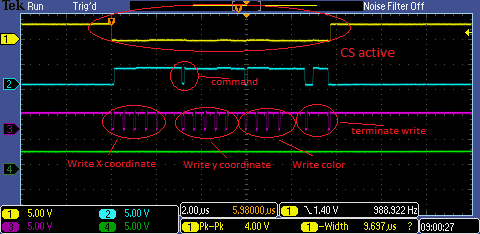
\includegraphics[width=0.8\textwidth]{pixel_write}
\caption{Writing one pixel to the display, including write termination.}
\label{fig:10}
\end{figure}

To complete writing one pixel data, write sequences are needed.
First there are five bytes written to set the X coordinate, then there are five bytes written for the Y coordinate. After that there are four bytes written for the color. At last, the write terminate command is written and CS is brought high. The first byte of each write sequence is the command, so the C/D line is low. When writing the other data the C/D line is high. The next four bytes of the coordinates are as follows: X/Y start coordinate (two bytes), X/Y end coordinate (two bytes). The color bytes are specified in red, green and blue.

Because writing a pixel takes about 10 $\mu$s, you can write about 100000 pixels per second.

\subsubsection{Reading pixel data from the display}
Reading a pixel is started by writing the pixel coordinate. After that, four bytes are read. The first byte read in is useless information, and the next three bytes are the color information in red, green and blue. After that, a read terminate is issued.

\begin{figure}[!ht]
\centering
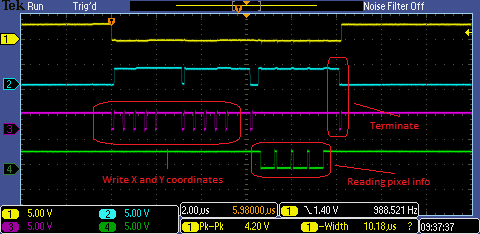
\includegraphics[width=0.8\textwidth]{pixel_read}
\caption{Reading one pixel to the display, includes termination.}
\label{fig:11}
\end{figure}

\subsubsection{Write and read pulse delay}
Please note that reading informations takes up more time that writing information. This is because the write and write pulse width need to be different. For a write the pulse width has to be 66 ns and for a read the pulse has to be 450 ns. Figure~\ref{fig:12} shows the difference.

\begin{figure}[!ht]
\centering
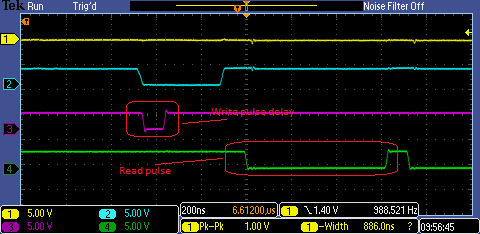
\includegraphics[width=0.8\textwidth]{write_read_delay}
\caption{The write and read pulse delay.}
\label{fig:12}
\end{figure}

In this setup, the write pulse delay is about 96 ns and the read pulse delay is about 620 ns, so there is some room for speeding up the write and read. This is because the automatic calculations of the delays is somewhat pessimistic \textsl{and} for writing and reading, the setup of the individual data and control signals takes some time. If you want to experiment with the pulse widths, please see $\S$~\ref{sec:writedelay} and $\S$~\ref{sec:readdelay}, but you may wind up with a non-responsive display. If this happens, just restore the original values and you'll be fine.


\subsection{Touchscreen timing diagrams}
The touchscreen is constructed with resistive foils, commenly named \textsl{plates}. As seen from the VMA412, the widest plate is called the x plate and de smaller plate is called the y plate. Because Arduino based software rotates the display 90$^\circ$ counter clockwise, x and y are swapped on these platforms.

Reading the x and y touched positions involves activating the plate to be read and then sample an analog voltage which indicates the point of touching. This is in electronic science called a \textsl{voltage divider}.

\subsubsection{Reading raw x}
To read the raw x position, XP is set high (about~3.3~V) and XM is set low (0~V). Then the voltage is read from YM. A low (digital) value indicates that the point of touching is more on the left (as positioned on the STM32) and a high (digital) value indicates that the point of touching is on the right. This value is an \textsl{indication} of where the plate is touched so you have to calculate the real display x coordinate. A sample of reading the raw x value is shown in Figure~\ref{fig:21}. Reading the raw X value takes about 30 $\mu$s because it is sampled 16 times (default) and the the mean of the samples is returned as digital value. Note that the mean is \textsl{not} the same as the average. Also, after reading the x value, a pixel is writte to the display to show the CS line is low. (This was needed to trigger the oscilloscope correctly.)

\begin{figure}[!ht]
\centering
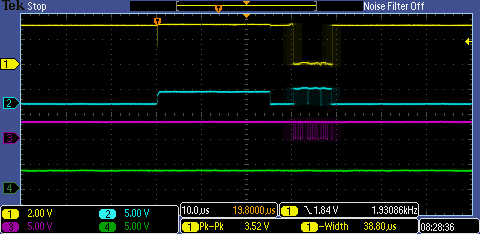
\includegraphics[width=0.8\textwidth]{sample_x}
\caption{Reading raw x.}
\label{fig:21}
\end{figure}

\subsubsection{Reading raw y}
Reading the raw y value is identical but now YP is set high, XM is set low and the analog voltage is read from XP. This is shown in Figure~\ref{fig:22}. Reading the raw y value also takes up about 30 $\mu$s.

\begin{figure}[!ht]
\centering
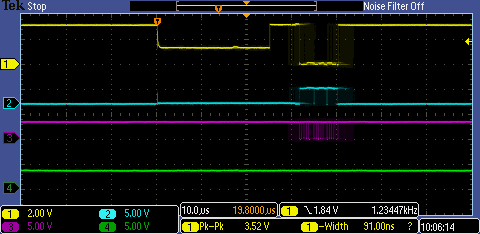
\includegraphics[width=0.8\textwidth]{sample_y}
\caption{Reading raw y.}
\label{fig:22}
\end{figure}


\subsubsection{Reading pressure}
Reading the pressure is more tricky, because there no plate for reading this value. Because of this the x and y plate are wired up together to get an indication of the pressure, and it is not possible to read the pressure accurately. For reading the pressure, XM is set high, YP is set low, and the pressure indication is read from both XP and YM. The \textsl{difference} of XP and YM is an indication of the pressure. In Figure~\ref{fig:26}, a complete reading of pressure, raw x and and raw y is shown. Reading the pressure involves reading two analog values and takes up 60 $\mu$s. This means that a complete reading of pressure, raw x and raw y takes up 120 $\mu$s.

\begin{figure}[!ht]
\centering
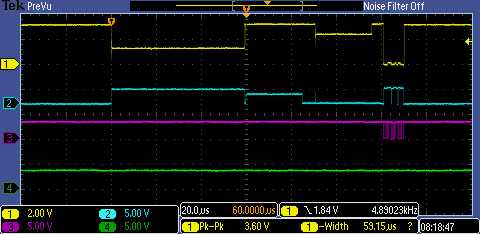
\includegraphics[width=0.8\textwidth]{sample_pressure_x_y}
\caption{Reading pressure, raw x and\textbf{} raw y in sequence.}
\label{fig:26}
\end{figure}

Because of the analog circuitry, after setting up the voltage across a plate, the analog inputs have to stabilize for about 400 to 800 ns. This is done automatically by the library.

When the raw values have read in from the analog inputs, you have to map these values to display coordinates. This is done by the function \lstinline|touchscreen_map| (see~$\S$~\ref{sec:touchmap}). First you have to figure out the minimum and maximum of the raw x and y values. The values have to be assigned to \lstinline|TOUCH_LEFT|, \lstinline|TOUCH_RIGHT|, \lstinline|TOUCH_TOP| and \lstinline|TOUCH_BOTTOM|. For deciding if the touchscreen is pressed you have to assign \lstinline|TOUCH_PRESSURE_LOW| and \lstinline|TOUCH_PRESSURE_HIGH|. A value below \lstinline|TOUCH_PRESSURE_LOW| or above \lstinline|TOUCH_PRESSURE_HIGH| is considered that the touchscreen is not pressed. The default values will suffice for most VMA412's.


\section{Library size}
If you compile the library functions into a static library, including internal font and THUAS bitmaps, the size of the static library is~63~kB when compiled with \lstinline|-Ofast| and~43~kB when compiled with \lstinline|-Os| (size optimized). If you disable the THUAS bitmaps, you save about~5~kB. Depending on the functions you use, the total added code to your code will be less than~63~kB. Alternative fonts are external and not considered in this calculations. 

\section{Todo's}
Some todo's left:

\begin{itemize}
\item Exchange display top/bottom or left/right (not rotating);
\item Make C++ wrappers;
\item Make C++ wrappers for AdaFruit based software (mostly Arduino sketches). This will be a separate project. This should minimize porting Arduino based software. One problem is that some functions are currently not implemented in this library. Also the Arduino based software rotates the display 90$^\circ$ with respect to this library, and swap X and Y readings from the touchscreen.
\item High-level touchscreen X and Y read functions (needs rotation information \textsl{and} GLCD functions for getting width and height);
\item Make code files Doxygen-proof;
\end{itemize}

This list will grow over time, and items implemented will be removed.

%% Add index to toc with clickable reference
\phantomsection
\addcontentsline{toc}{section}{\indexname}

\printindex


\end{document}
